\documentclass[12pt,a4paper]{report}

\usepackage[top=1in, bottom=1in, left=1.25in, right=1.25in]{geometry}
\usepackage{graphicx}
\usepackage{float}
% \usepackage{xeCJK}
\usepackage{ctex}
% \setCJKmainfont{FangSong}
\setCJKmainfont{KaiTi}
\usepackage{algorithm}
\usepackage{algorithmicx}
\usepackage{algpseudocode}
\usepackage{listings}
\usepackage{color}
\usepackage{tikz}
\usepackage{fancyhdr}
\usepackage{amsmath,amssymb,amsthm}
\usepackage[toc,page]{appendix}
\usepackage{multirow}
\usepackage[utf8]{inputenc}
\usepackage{booktabs}

\definecolor{mygreen}{rgb}{0,0.6,0}
\definecolor{mygray}{rgb}{0.5,0.5,0.5}
\definecolor{mymauve}{rgb}{0.58,0,0.82}

\algblockdefx{MRepeat}{EndRepeat}{\textbf{repeat}}{}
\algnotext{EndRepeat}

\lstset{
	language=C,
	numbers=left,
	breaklines=true,
	basicstyle=\scriptsize,
	commentstyle=\color{mygreen},
	keywordstyle=\color{blue},
	numberstyle=\color{mygray},
	rulecolor=\color{black},
	stringstyle=\color{mymauve}
}

\pagestyle{fancy}
\lhead{\leftmark}
\rhead{Course Summary}
\renewcommand{\headrulewidth}{0.5pt}

\title{
	
\includegraphics[scale=1.5]{1.png}\\~\\
	
\includegraphics[scale=1.5]{2.png}\\
	~\\
	\Huge\textbf{上课内容总结}\\
	\large\textbf{Introduction of Applied Operations Research}\\
}
\author{
	许子骏\\
	\texttt{3160100056}
	\\ 计算机科学与技术1603
}

\begin{document}
	\maketitle
	\tableofcontents

	\chapter{线性规划}
\section{相关定义}
\subsection{凸集及凸函数}
\subsubsection{凸集}
对于集合 $S$,若任意两元素 $x, y \in S$,且对于任意 $0 \le \theta \le 1$ 有 
$$
\theta x + (1-\theta)y \in S
$$
则 $S$ 是凸集 (convex set)。 \\~\\
可以推广:若 $S$ 为凸集, 
$$
\sum_{i=1}^n \theta_ix_i \in S \\
$$
$$
\begin{cases}
x_1, x_2, \dots, x_n \in S, \  \forall n \ge 2 \\
\forall \sum_{i=1}^n \theta_i = 1
\end{cases}
$$

\subsubsection{凸函数}
对于定义在凸集 $S$ 上的函数 $f(x)$,若对于 $\forall 0 \le \theta \le 1$ 有
$$
f(\theta x + (1-\theta) y) \le \theta f(x) + (1-\theta) f(y)
$$
则 $f(x)$ 是凸函数 (convex function)。 \\~\\
若 $f(x)$ 是凸函数,
$$
f(\sum_{i=1}^n \theta_ix_i) \le \sum_{i=1}^n \theta_i f(x_i), \ \forall \sum_{i=1}^n \theta_i = 1
$$
若 $-f(x)$ 是凸函数,则 $f(x)$ 是凹函数(concave function);根据定义,仿射函数 (affine function) 既是凸函数也是凹函数。 \\~\\
对于所有凸函数,\textbf{局部最优就是全局最优}。

\subsection{线性规划}
线性规划(linear programming, LP)问题指的是如下形式的优化问题:
$$
\max \quad c^Tx \\
$$
$$
\text{s.t.} 
\begin{cases}
    Ax = b \\ 
    x \ge 0    
\end{cases}
$$
简单来说,就是目标函数和约束函数都是仿射函数的优化问题。

\subsubsection{极点}
设 $S$ 为凸集,若 $x \in S$ 无法表示为其它两个 $S$ 内元素的凸组合,则 $x$ 是极点 (extreme point)。

\subsubsection{基可行解}
假设 $A$ 是一个 $m \times n$ 的矩阵,我们讨论 $Ax = b$ 有解且 $A$ 行满秩的情况,可以从 $A$ 中选出最多 $m$ 列线性无关的列向量,其它列向量都和它们线性相关,把 $A$ 分成 $\begin{bmatrix} A_B & A_N \end{bmatrix}$ ,其中 $A_B$ 就是那 $m$ 个线性无关的列向量。 \\
我们容易构造出 $Ax = b$ 的一个解:
$$x = \begin{bmatrix} A_B^{-1}b \\ 0 \end{bmatrix}$$ 
称这种解为基可行解 (basic feasible solution)。显然,基可行解至多有 $C_n^m$ 种。 \\~\\ 
基可行解有个重要的性质:\textbf{每个极点都对应着一个基可行解,且每个基可行解都对应着一个极点}。

\pagebreak

\section{单纯形法}
\subsection{单纯形法}
单纯形法 (simplex method) 的每一步都在引入一个非基变量取代某一基变量,找出目标函数值更优的另一基本可行解,逐渐调整到最优解。 \\
有以下步骤:
\begin{enumerate}
    \item 把线性规划问题的约束方程组表达成典范型方程组,找出基本可行解作为初始基可行解。
    \item 若基本可行解不存在,即约束条件有矛盾,则问题无解。
    \item 若基本可行解存在,从初始基可行解作为起点,根据最优性条件和可行性条件,引入非基变量取代某一基变量,找出目标函数值更优的另一基本可行解。
    \item 按步骤3进行迭代,直到对应检验数满足最优性条件(这时目标函数值不能再改善),即得到问题的最优解。
    \item 若迭代过程中发现问题的目标函数值无界,则终止迭代。
\end{enumerate}
假设有以下问题:
$$
\max \quad 3x_1 + 2x_2
$$
$$
\text{s.t.} 
\begin{cases}
    2x_1 + x_2 \le 12 \\
    x_1 + 2x_2 \le 9 \\
    x_1, x_2 \ge 0
\end{cases}
$$
加入松弛变量,将原问题变为 
$$
\max \quad 3x_1 + 2x_2
$$
$$
\text{s.t.} 
\begin{cases}
    2x_1 + x_2 + x_3 = 12 \\
    x_1 + 2x_2 + x_4 = 9 \\
    x_1, x_2, x_3, x_4 \ge 0
\end{cases}
$$
此时,有初始可行解:$x = \begin{bmatrix} 0 & 0 & 12 & 9 \end{bmatrix}^T$,当前目标函数值为 $z = 0$。将各个变量用非基变量进行表示,有
$$
\begin{cases}
    x_3 = 12 - 2x_1 - x_2 \\ 
    x_4 = 9 - x_1 - 2x_2 \\ 
    z = 3x_1 + 2x_2
\end{cases}
$$
$x_1$ 的系数比较大(这个系数称为\textbf{检验数}),将 $x_1$ 变成基变量。根据 $x_1$ 与 $x_3$ 和 $x_4$ 之间的表达式不难看出,当 $x_1 = 6$ 时,$x_3$ 最先变成 0,将它从基变量中去除。
此时,可行解变为 $x = \begin{bmatrix}6 & 0 & 0 & 3\end{bmatrix}^T$,当前目标函数值为 $z = 18$。将各个变量用非基变量进行表示,有
$$
\begin{cases}
x_1 = 6 - x_2/2 - x_3/2 \\ 
x_4 = 3 - 3x_2/2 + x_3/2 \\ 
z = 18 + x_2/2 - 3x_3/2
\end{cases}
$$
从系数可以看出,只有增加 $x_2$ 才能增大目标函数值,将 $x_2$ 变成基变量。从 $x_2$ 与 $x_1$ 和 $x_4$ 的关系式中也不难发现,当 $x_2 = 2$ 时,$x_4$ 最先变成 0,我们把它从基变量中去除。
此时,可行解变为 $x = \begin{bmatrix} 5 & 2 & 0 & 0 \end{bmatrix}^T$,当前目标函数值为 $z = 19$。将各个变量用非基变量进行表示,有 
$$
\begin{cases}
x_1 = 5 - 2x_3/3 + x_4/3 \\ 
x_2 = 2 + x_3/3 - 2x_4/3 \\ 
z = 19 - 4x_3/3 - x_4/3
\end{cases}
$$
可以发现,$x_3$ 和 $x_4$ 与 $z$ 相关的系数都是负值,此时无论把哪个变量加入基变量,都只能让目标函数值变小了。此时得到了线性规划问题的最优解:$x = \begin{bmatrix} 5 & 2 & 0 & 0 \end{bmatrix}^T$,目标函数值为 $z = 19$。

\subsection{单纯形表}
单纯形表 (simplex tableau) 用矩阵的形式,将单纯形法中各个变量用非基变量进行表示。
假设有以下线性规划问题:
$$
\max \quad z = c^Tx
$$
$$
\text{s.t.} 
\begin{cases}
    Ax \le b \\
    x \ge 0
\end{cases}
$$
将各个矩阵或向量根据基变量和非基变量分为两部分:
令 $c^T = \begin{bmatrix} c_B^T & c_N^T \end{bmatrix}, A = \begin{bmatrix} A_B & A_N \end{bmatrix}, x = \begin{bmatrix} x_B^T & x_N^T \end{bmatrix}^T$,有
$$
\begin{cases}
A_Bx_B + A_Nx_N = b \\ 
z = c_B^Tx_B + c_N^Tx_N
\end{cases}
$$
通过移项就能用 $x_N$ 表示其它变量:
$$
\begin{cases}
x_B = A_B^{-1}b - A_B^{-1}A_Nx_N \\ 
z = c_B^TA_B^{-1}b + (c_N^T - c_B^TA_B^{-1}A_N)x_N
\end{cases}
$$
由于基可行解中 $x_N = 0$,有
$$
\begin{cases}
x_B = A_B^{-1}b \\ 
z = c_B^TA_B^{-1}b
\end{cases}
$$
首先画一张这样的表:
$$
\begin{array}{c|cc|c} & c_B^T & c_N^T & 0 \\ \hline x_B & A_B & A_N & b\end{array}
$$
利用行变换将 $A_B$ 变为 $I$,有
$$
\begin{array}{c|cc|c} & c_B^T & c_N^T & 0 \\ \hline x_B & I & A_B^{-1}A_N & A_B^{-1}b\end{array}
$$
接着把下面一行乘上 $c_B^T$,用上面一行相减,有
$$
\begin{array}{c|cc|c} & 0 & c_N^T-c_B^TA_B^{-1}A_N & -c_B^TA_B^{-1}b \\ \hline x_B & I & A_B^{-1}A_N & A_B^{-1}b\end{array}
$$
表格每计算一次,即为单纯形法的一次迭代。 \\~\\
假设有以下问题:(和上一节例子相同)
$$
\max \quad 3x_1 + 2x_2
$$
$$
\text{s.t.} 
\begin{cases}
    2x_1 + x_2 \le 12 \\
    x_1 + 2x_2 \le 9 \\
    x_1, x_2 \ge 0
\end{cases}
$$
加入松弛变量后,有
$$
\max \quad 3x_1 + 2x_2
$$
$$
\text{s.t.} 
\begin{cases}
    2x_1 + x_2 + x_3 = 12 \\
    x_1 + 2x_2 + x_4 = 9 \\
    x_1, x_2, x_3, x_4 \ge 0
\end{cases}
$$
初始单纯形表:
$$
\begin{array}{c|cccc|c} & 3 & 2 & 0 & 0 & 0 \\ \hline x_3 & 2 & 1 & 1 & 0 & 12 \\ x_4 & 1 & 2 & 0 & 1 & 9 \end{array}
$$
选择检验数中较大的那个($3$,对应 $x_1$)。由于 $12/2 = 6 < 9/1 = 9$,所以 $x_1$ 成为基变量,$x_3$ 被移出基变量。修改表格为
$$
\begin{array}{c|cccc|c} & 0 & 1/2 & -3/2 & 0 & -18 \\ \hline x_1 & 1 & 1/2 & 1/2 & 0 & 6 \\ x_4 & 0 & 3/2 & -1/2 & 1 & 3 \end{array}
$$
选择最大的检验数($1/2$,对应 $x_2$),由于 $3/(3/2) = 2 < 6/(1/2) = 12$,所以 $x_2$ 成为基变量,$x_4$ 被移出基变量。修改表格为
$$
\begin{array}{c|cccc|c} & 0 & 0 & -4/3 & -1/3 & -19 \\ \hline x_1 & 1 & 0 & 2/3 & -1/3 & 5 \\ x_2 & 0 & 1 & -1/3 & 2/3 & 2 \end{array}
$$
此时所有检验数都为非正数,单纯形法结束。单纯形表右上角的 $-z$ 就是最优目标函数的相反数,所以最优目标函数为 $19$。表格最右一列的 $A_B^{-1}b$ 就是 $x_B$ 的取值,所以最优解为 $x_1 = 5$,$x_2 = 2$。

\subsection{退化}
退化 (degeneration) 指一个基可行解中,存在至少一个基变量为 $0$ 的情况,即这个基变量可以和另一个非基变量任意互换,而不影响结果。 \\
可以通过以下规则,避免单纯形法进入循环:\textbf{在有多个可以入基的变量时,选择下标最小的一个;在有多个可以出基的变量时,也选择下标最小的一个}。 \\
接下来证明\textbf{单纯形法在非退化的情况下必定可以取到最优解}: \\~\\
首先证明:若检验数向量 $\hat{c} = c_N - c_B^TA_B^{-1}A_N$ 的每一维都小等于 $0$,那么此时基可行解 $x$ 是最优解。 \\
利用反证法,假设有一个更优的 $y$ 才是最优解。令 $d = x - y$,我们有 
$$
Ax - Ay = b - b = 0 = Ad = A_Bd_B + A_Nd_N
$$
令 $d_B = -A_B^{-1}A_Nd_N$ 则
$$
c^Td = c_B^Td_B + c_N^Td_N = (c_N^T-c_B^TA_B^{-1}A_N)d_N = \hat{c}d_N
$$
根据基可行解的定义 $x_N = 0$,又 $y \ge 0$,因此 $d_N \ge 0$;又 $\hat{c} \le 0$,所以 $c^Td = \hat{c}d_N \le 0$,则 $c^Ty = c^Tx + c^Td \le c^Tx$,说明 $y$ 并没有比 $x$ 更优,矛盾。这说明了在检验数均小等于 $0$ 时停止算法,就能得到最优解。 \\
类似地,可以说明若基可行解 $x$ 是非退化的最优解,检验数向量的每一维都小等于 $0$。否则由于 $x$ 是非退化的最优解,如果有一个检验数大于 $0$,它对应的非基变量一定有增加的空间,就能构造一个更优的解。这说明了在非退化的情况下,肯定有解满足算法停止的情况。

\subsection{大M法}
大M法 (big M method)将线性规划的目标函数改为
$$
z = c^Tx - M\sum_{i=1}^m\bar{x}_i
$$
如果 $M$ 是一个足够大的正数,如果原问题存在可行解,$\bar{x}$ 就会在 $-M$ 这个“惩罚”之下变成 $0$。
然而, $M$ 的值无从定义。如果 $M$ 的值取得太小导致 $\bar{x}$ 最后仍非 $0$,此时,有两种可能,一是 $M$ 太小了,另一个则是因为问题没有可行解;如果 $M$ 的值取得太大,可能会带来计算上的误差。

\subsection{两阶段法}
两阶段法 (two-phase metehod) 将原问题改变为只由松弛变量组成的优化问题,解决了这个优化问题,就找到了原问题的一个可行解。 \\
有优化问题如下:
$$
\min \quad \sum_{i = 1}^{m} \bar{x}_i
$$
$$
\text{s.t.} 
\begin{cases}
    Ax + \bar{x} = b \\
    x, \bar{x} \ge 0
\end{cases}
$$
对于这个优化问题,$\bar{x} = b$ 就是一个可行解。 \\
如果这个优化问题的最优解的目标函数值不为 $0$,原问题无可行解;如果最优解让目标函数值为 $0$,则存在一种 $x$ 的取值满足约束,且 $\bar{x} = 0$,这样就找到了原问题的一个可行解。再以这个可行解为起点,利用单纯形法求出原问题的最优解即可。 \\~\\
假设有以下问题:
$$
\max \quad 4x_1 - x_2 + x_3
$$
$$
\text{s.t.} 
\begin{cases}
    x_1 + 2x_2 + 3x_3 = 1 \\
    2x_1 + 3x_2 + 2x_3 = 2 \\
    x \ge 0
\end{cases}
$$
加入松弛变量后,转化为两阶段法的优化问题:
$$
\max \quad -x_4 - x_5
$$
$$
\text{s.t.} 
\begin{cases}
    x_1 + 2x_2 + 3x_3 + x_4 = 1 \\
    2x_1 + 3x_2 + 2x_3 + x_5 = 2 \\
    x \ge 0
\end{cases}
$$
初始单纯形表:
$$
\begin{array}{c|ccccc|c} & 3 & 5 & 5 & 0 & 0 & 3 \\ \hline x_4 & 1 & 2 & 3 & 1 & 0 & 1 \\ x_5 & 2 & 3 & 2 & 0 & 1 & 2\end{array}
$$
选择 $x_1$ 入基,$x_4$ 出基,有
$$
\begin{array}{c|ccccc|c} & 0 & -1 & -4 & -3 & 0 & 0 \\ \hline x_1 & 1 & 2 & 3 & 1 & 0 & 1 \\ x_5 & 0 & -1 & -4 & -2 & 1 & 0 \end{array}
$$
此时,目标函数值已经是 $0$ 了,但是基变量里有一个 $x_5$,这是一个退化情况,我们有 $x_2 = x_3 = x_5 = 0$。此时可以让 $x_2$ 入基,$x_5$ 出基,就能把基变量变为 $x_1$ 和 $x_2$。同时也求出了原问题的一个可行解:$x_1 = 1, x_2 = x_3 = 0$,基变量是 $x_1$ 和 $x_2$。 \\
利用单纯形表求解原问题,有初始单纯形表:
$$
\begin{array}{c|ccc|c} & 0 & 0 & 25 & -4 \\ \hline x_1 & 1 & 0 & -5 & 1 \\ x_2 & 0 & 1 & 4 & 0 \end{array}
$$
这一个退化情况。让 $x_3$ 入基,$x_2$ 出基,有
$$
\begin{array}{c|ccc|c} & 0 & -25/4 & 0 & -4 \\ \hline x_1 & 1 & 5/4 & 0 & 1 \\ x_3 & 0 & 1/4 & 1 & 0 \end{array}
$$
所有检验数都非正,迭代结束。得到了原问题的最优解:$x_1 = 1, x_2 = x_3 = 0$,此时目标函数值为 $4$。
\pagebreak

\section{对偶理论}
\subsection{对偶问题}
对于一个线性规划问题(称为原问题,primal,记为 P)
$$
\max \quad c^Tx
$$
$$
\text{s.t.} 
\begin{cases}
    Ax \le b \\
    x \ge 0
\end{cases}
$$
定义它的对偶问题(dual,记为 D)为
$$
\min \quad b^Ty
$$
$$
\text{s.t.} 
\begin{cases}
    A^Ty \ge c \\
    y \ge 0
\end{cases}
$$
这里的对偶变量 $y$,可以看作是对原问题的每个限制,都用一个变量来表示。 \\~\\
原问题限制条件的不等号,和对偶问题限制条件的不等号,是相互关联的。假设原问题是一个最大化问题,设 $a_i^T$ 表示 $A$ 中的第 $i$ 行,我们有以下结论:
\begin{enumerate}
    \item $a^Tx \_ bx$ 和 $y_i \_ 0$ 关系:
    \begin{table}[!htbp]
        \centering
        \begin{tabular}{|c|c|c|}
            \hline 
            \multicolumn{2}{|c|}{} & $y_i \_ 0$ \\
            \hline
            \multirow{3}*{$a^Tx \_ bx$} & $\le$ & $\ge$ \\
            \cline{2-3}
            & $\ge$ & $\le$ \\
            \cline{2-3}
            & = & 无限制 \\
            \hline
        \end{tabular}
    \end{table}
    \item $x_i \_ 0$ 和 $A^T_iy \_ c_i$ 关系:
    \begin{table}[!htbp]
        \centering
        \begin{tabular}{|c|c|c|}
            \hline 
            \multicolumn{2}{|c|}{} & $A^T_iy \_ c_i$ \\
            \hline
            \multirow{3}*{$x_i \_ 0$} & $\ge$ & $\ge$ \\
            \cline{2-3}
            & $\le$ & $\le$ \\
            \cline{2-3}
            & 无限制 & = \\
            \hline
        \end{tabular}
    \end{table}
\end{enumerate}

\subsection{对偶问题的性质}
\subsubsection{对称性}
对称性 (symmetry),即假设有原问题,以及其对偶问题,则其\textbf{对偶问题的对偶问题即原问题}。 \\
将对偶问题变成标准形式,有
$$
\max \quad y^T(-b)
$$
$$
\text{s.t.} 
\begin{cases}
    (-A^T)y \le -c \\
    y \ge 0
\end{cases}
$$
它的对偶问题是
$$
\min \quad -c^Tx
$$
$$
\text{s.t.} 
\begin{cases}
    -Ax \ge -b \\
    x \ge 0
\end{cases}
$$
把目标函数和限制都乘以 $-1$ 后即原问题。

\subsubsection{弱对偶定理}
弱对偶定理 (weak duality),即假设 $x$ 和 $y$ 分别是原问题和对偶问题的可行解,有 \textbf{$c^Tx \le b^Ty$}。 \\
由 $y$ 的可行性,有 $A^Ty \ge c$,即 $y^TA \ge c^T$,两边同乘以 $x$ ,有 $y^TAx \ge c^Tx$;由 $x$ 的可行性,有 $Ax \le b$,则 $y^TAx \le y^Tb$,合起来就是 $c^Tx \le b^Ty$。

\subsubsection{最优性}
最优性 (optimality),即假设 $x$ 和 $y$ 分别是原问题和对偶问题的可行解,且 $c^Tx = b^Ty$,那么 $x$ 和 $y$ 分别是原问题和对偶问题的最优解。

\subsubsection{无界性}
无界性 (unbounded),即
\begin{enumerate}
    \item 若原问题有可行解无最优解(目标函数值可以取无穷大),则对偶问题无可行解。
    \item 若对偶问题有可行解无最优解,则原问题无可行解。
\end{enumerate}

\subsubsection{强对偶定理}
强对偶定理 (strong duality),即\textbf{若原问题(或对偶问题)有有限最优解,则对偶问题(或原问题)也有有限最优解,且最优解相等}。
以下通过通过单纯形法的计算过程辅助证明: \\~\\~\\
假设加上松弛变量后,原问题变为
$$
\max \quad c^Tx
$$
$$
\text{s.t.} 
\begin{cases}
    \bar{A}x = b \\
    x \ge 0
\end{cases}
$$
有初始单纯形表
$$
\begin{array}{c|cc|c} & c^T & 0 & 0 \\ \hline x^*_B & A & I & b \end{array}
$$
最终单纯形表为
$$
\begin{array}{c|cc|c} & c^T - c^T_B\bar{A}_B^{-1}A & -c^T_B\bar{A}_B^{-1} & -c^T_B\bar{A}_B^{-1}b \\ \hline x^*_B & \bar{A}_B^{-1}A & \bar{A}_B^{-1} & \bar{A}_B^{-1}b \end{array}
$$
由于 $x^*_B$ 是原问题最优的基变量组合,则检验数均非正,有
\begin{align}
& c^T \le c^T_B\bar{A}_B^{-1}A \tag{1} \\
& -c^T_B\bar{A}_B^{-1} \le 0 \tag{2}
\end{align}
取 $y^{*T} = c^T_B\bar{A}_B^{-1}$,代入以上条件$(1)$和$(2)$,有 $A^Ty^* \ge c$ 和 $y^* \ge 0$,即 $y^*$ 是一个可行解。 \\
根据单纯形法,有 $x^*_B = \bar{A}_B^{-1}b$,$x^*_N = 0$,则对偶问题的目标函数值为 $b^Ty^* = y^{*T}b = c^T_B\bar{A}_B^{-1}b = c^T_Bx^*_B = c^Tx^*$,为一对可行的 $x$ 和 $y$,使得原问题和对偶问题的目标函数值相等。 \\
根据弱对偶定理,这两个可行解分别是原问题和对偶问题的最优解。

\subsubsection{互补松弛定理}
互补松弛定理 (complementary slackness),即假设 $x^*$ 与 $y^*$ 分别是原问题和对偶问题的可行解,以下条件等价:
\begin{enumerate}
    \item $x^*$ 和 $y^*$ 分别是原问题和对偶问题的最优解。
    \item $(y^{*T}A - c^T)x^* = 0$ 且 $y^{*T}(Ax^*-b) = 0$。
\end{enumerate}
有以下证明: \\
$1 \Rightarrow 2$: \\
$y^{*T}b = y^{*T}Ax^* = c^Tx^*$,根据弱对偶定理得 $x^*$ 和 $y^*$ 分别是原问题和对偶问题的最优解。 \\
$2 \Rightarrow 1$: \\
根据弱对偶定理的推导,有 $y^{*T}b \ge y^{*T}Ax^* \ge c^Tx^*$。因为 $x^*$ 和 $y^*$ 分别是原问题和对偶问题的最优解,有 $y^{*T}b = c^Tx^*$,则  $y^{*T}b = y^{*T}Ax^* = c^Tx^*$,即$(y^{*T}A - c^T)x^* = 0$ 且 $y^{*T}(Ax^*-b) = 0$。

\subsection{对偶单纯形法}
对单纯形法的停止条件是所有检验数非正($max$ 问题,若是 $min$ 问题所有检验数非负),根据强对偶定理的推导,当所有检验数非正,此时能构造一个对偶问题的可行解,使得原问题和对偶问题的目标函数值相等,则这两目标函数值分别是原问题和对偶问题的最优解。\\ 
即保证原问题可行解的情况下,尝试构造对偶问题的可行解,如果构造成功,则两个目标函数值都是最优解。 \\
相应地,在保证对偶问题可行解($max$ 问题所有检验数非正, 若是 $min$ 问题所有检验数非负)的情况下,尝试构造原始问题的可行解,如果构造成功,则两个目标函数值都是最优解。 \\
这种单纯形法的变型又称为对偶单纯形法 (dual simplex method)。 \\
对于$min$问题,有以下步骤:
\begin{enumerate}
    \item 找到一组基,使得所有检验数非负。
    \item 若单纯形表中 $b$ 的那一列出现负数,因为有 $x \ge 0$ 的限制,当前基不可行,选择负数中 $b$ 的绝对值最大的那一行(设为第 $i$ 行),对应的变量 $x_i$ 作为出基变量(需将该变量从负数变换为 0)。
    \item 假设第 $i$ 行中,$x_j$ 的系数为 $a_j$,检验数为 $d_j$,则在所有 $a_j < 0$ 的变量中,选择 $d_j/a_j$ 绝对值最小的那一列,对应的变量 $x_k$ 作为入基变量,回到 步骤 $2$。如果所有 $a_j \ge 0$,则原问题无可行解。
    \item 若单纯形表中 $b$ 的那一列均非负,即构造出了一个原问题的可行解,算法结束。
\end{enumerate}
假设有以下问题:
$$
\min \quad 9x_1 + 5x_2 + 3x_3
$$
$$
\text{s.t.} 
\begin{cases}
    3x_1 + 2x_2 - 3x_3 \ge 3 \\
    2x_1 + x_3 \ge 5 \\
    x \ge 0
\end{cases}
$$
加入松弛变量后,问题转化为
$$
\min \quad 9x_1 + 5x_2 + 3x_3
$$
$$
\text{s.t.} 
\begin{cases}
    3x_1 + 2x_2 - 3x_3 - x_4 = 3 \\
    2x_1 + x_3 - x_5 =  5 \\
    x \ge 0
\end{cases}
$$
有初始单纯形表
$$
\begin{array}{c|ccccc|c} & 9 & 5 & 3 & 0 & 0 & 0 \\ \hline x_4 & -3 & -2 & 3 & 1 & 0 & -3 \\ x_5 & -2 & 0 & -1 & 0 & 1 & -5 \end{array}
$$
选择 $x_5$ 出基. 由于 $3/1 < 9/2$,选择 $x_3$ 入基,有
$$
\begin{array}{c|ccccc|c} & 3 & 5 & 0 & 0 & 3 & -15 \\ \hline x_4 & -9 & -2 & 0 & 1 & 3 & -18 \\ x_3 & 2 & 0 & 1 & 0 & -1 & 5 \end{array}
$$
选择 $x_4$ 出基. 由于 $3/9 < 5/2$,选择 $x_1$ 入基,有
$$
\begin{array}{c|ccccc|c} & 0 & 13/3 & 0 & 1/3 & 4 & -21 \\ \hline x_1 & 1 & 2/9 & 0 & -1/9 & -1/3 & 2 \\ x_3 & 0 & -4/9 & 1 & 2/9 & -1/3 & 1 \end{array}
$$
此时最后一列第二、三行均非负,迭代结束。原问题的最优解为 $x_1 = 2, x_2 = 0, x_3 = 1$,目标函数值为 $21$。

\subsection{原始对偶方法}
假设已知对偶问题的可行解 $y$ ,需要寻找一个原问题的可行解 $x$ 满足互补松弛定理。
假设 $A_j$ 表示矩阵 $A$ 的第 $j$ 列,定义 $J = \{ j | A_j^Ty = c_j \}$(称 $J$ 为允许指标集)。根据原问题的定义和互补松弛定理,有
\begin{align}
& Ax = b \tag{1} \\ 
& x_j = 0 \quad \forall j \not\in J \tag{2} \\ 
& x_j \ge 0 \quad \forall j \in J \tag{3}
\end{align}
如果能找到一个 $x$ 满足上面三个条件,$x$ 和 $y$ 就能满足互补松弛定理。 \\
为了获得一个可行的 $x$,构造一个优化问题,称为限制的原问题(restricted primal, RP)。
$$
\max \quad \sum_{i = 1}^m \bar{x_i}
$$
$$
\text{s.t.} 
\begin{cases}
    \sum_{j \in J} a_{i, j}x_j + \bar{x_i} = b_i \\
    x_j \ge 0, \bar{x_i} \ge 0
\end{cases}
$$
若目标函数值取 $0$,则得到满足互补松弛定理的 $x$。
写出 RP 的对偶问题,称为限制的对偶问题(dual restricted primal, DRP)。 \\~\\ \pagebreak
$$
\max \quad b^Ty
$$
$$
\text{s.t.} 
\begin{cases}
    A^T_jy \le 0, \ \forall j \in J \\
    y_i \le 1, \ \forall i \in \{1, 2, \ \cdots, m\}
\end{cases}
$$
假设 $\bar{y}$ 为 DRP 的最优解,根据强对偶定理,若 $b^T\bar{y} = 0$ ,则 RP 的目标函数值也可以取 $0$,则当前对偶可行的 $y$ 就是对偶问题的最优解;否则有 $b^T\bar{y} \ge 0$,因为至少 $\bar{y} = 0$ 是 DRP 的可行解。 \\
如果发现 RP 问题无可行解,或者 DRP 问题无有限最优解,则原问题无可行解。 \\~\\
如果 DRP 的最优解让 DRP 的目标函数值超过 $0$,说明当前的 $y$ 还不是最优的。\\ 
假设新的对偶可行解 $\hat{y} = y + \theta\bar{y}$($\theta \ge 0$),有 $b^T\hat{y} = b^Ty + \theta b^T\bar{y} > b^Ty$,改进对偶问题的目标函数值。由于 $\hat{y}$ 仍然是对偶可行的,即必须满足 $A^T\hat{y} = A^Ty + \theta A^T\hat{y} \le c$ 。 \\
对于 $j \in J$,因为 $A^T_j\bar{y} \le 0$,无论 $\theta$ 取多大,都不会超过 $c$ 的限制;对于 $j \not\in J$,选择
$$
\theta = \min_{j \not\in J, A^T_j\bar{y} > 0} \quad \frac{c_j - A^T_jy}{A^T_j\bar{y}}
$$
使得 $j \not\in J$ 中的一条限制变紧,其它限制不会超过,仍然是对偶可行的。若 $\theta$ 可以无限增大,则对偶问题没有有限最优解,原问题无可行解。
将 $y$ 调整为 $\hat{y}$ 之后,进入下一轮迭代继续调整,直到 DRP 的最优解让目标函数值为 $0$,此时的 $y$ 就是对偶问题的最优解。

\subsubsection{应用:最短路问题}
考虑有向图上的最短路问题,起点为 $s$,终点为 $t$。对有向图定义点 - 弧关联矩阵,若一条边是一个顶点的出边,那么矩阵对应元素为 $1$;若一条边是一个顶点的入边,那么矩阵对应元素为 $-1$。假设 $w_i$ 表示第 $i$ 条边的长度,$x_i$ 表示第 $i$ 条边是否在最短路上,
可构造线性规划问题
$$
\min \quad w^Tx
$$
$$
\text{s.t.} 
\begin{cases}
    Ax = v \\
    x \ge 0
\end{cases}
$$
因为 $s$ 为起点,$t$ 为终点,
$$
v_i = \begin{cases} 1 & i = s \\ -1 & i = t \\ 0 & \text{otherwise} \end{cases}
$$
根据点 - 弧关联矩阵的定义很容易发现,把 $A$ 的每一行加起来,最后会获得都是 $0$ 的一行,即 $A$ 中的行向量线性相关。可从 $A$ 中去掉代表终点 $t$ 的那一行,得到新矩阵 $\bar{A}$。 \\
得到新的线性规划问题
$$
\min \quad w^Tx
$$
$$
\text{s.t.} 
\begin{cases}
    \bar{A}x = v \\
    x \ge 0
\end{cases}
$$
其中
$$
v_i = \begin{cases} 1 & i = s \\ 0 & \text{otherwise} \end{cases}
$$
写出对偶问题
$$
\max \quad \pi_s
$$
$$
\text{s.t.} 
\begin{cases}
    \pi_i - \pi_j \le w_e, \ \forall e = (i, j) \in E \\
    \pi_t = 0
\end{cases}
$$
只要令$\pi = 0$ 即可得到对偶问题的可行解。 \\
写出DRP
$$
\max \quad \pi_s
$$
$$
\text{s.t.} 
\begin{cases}
    \pi_i - \pi_j \le 0, \ \forall (i, j) \in J \\
    \pi_i \le 1 \\
    \pi_t = 0
\end{cases}
$$
如果已知从点 $s$ 到某点 $p$ 的最短路,而边 $j$ 就在这条最短路上,根据最短路的三角不等式,这条边一定在 $j$ 中。假设 $C$ 为已知最短路的点构成的连通块,为了让 $\pi_s$ 的取值最大并满足 DRP 的限制条件,$C$ 中所有点的变量值都必须和 $\pi_s$ 相同。若 $t \not\in C$, $\pi_s = 1$;若 $t \in C$,由于 $\pi_t = 0$ 的条件,$\pi_s = 0$,得到了从 $s$ 到 $t$ 的最短路。 \\~\\
假设有以下问题:
\begin{figure}[H]
    \begin{center}
        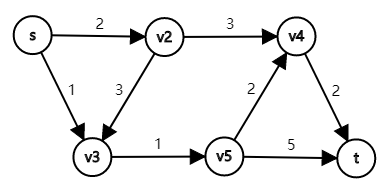
\includegraphics[scale=0.9]{img/drp_shortest_path.png}
        \caption{最短路问题例子。}
    \end{center}
\end{figure}
\begin{table}[!htbp]
    \centering
    \begin{tabular}{c|cccccc} 
        & $\pi_s$ & $\pi_{v_2}$ & $\pi_{v_3}$ & $\pi_{v_4}$ & $\pi_{v_5}$ & $\pi_t$ \\ 
        \hline 
        0 & 0 & 0 & 0 & 0 & 0 & 0 \\ 
        1 & 1 & 0 & 0 & 0 & 0 & 0 \\ 
        2 & 2 & 0 & 1 & 0 & 0 & 0 \\ 
        3 & 4 & 2 & 3 & 0 & 2 & 0 \\ 
        4 & 6 & 5 & 4 & 2 & 4 & 0
    \end{tabular}
    \caption{最短路问题例子迭代过程。}
    \label{table:drp_shortest_path}
\end{table}
绘制表格,记录每次迭代的 $\pi$ 值。通过表\ref{table:drp_shortest_path} ,经过 $4$ 次迭代,得到 $s$ - $t$ 的最短路为 $6$。

\pagebreak

	\chapter{组合优化}
\section{整数规划}
\subsection{整数规划}
整数规划就是线性规划加上解必须为整数的限制,其基本形式为
$$
\max \quad c^Tx
$$
$$
\text{s.t.} 
\begin{cases}
    Ax \le b \\
    x \in \mathbb{N}
\end{cases}
$$
常见的很多算法问题都能写成线性整数规划的形式,特别是能写成整数规划的一种特殊形式:$0 - 1$ 规划。

\subsubsection{$0 - 1$ 背包问题}
假设共有 $n$ 件物品,$v_i$ 表示第 $i$ 件物品的价值,$w_i$ 表示第 $i$ 件物品的重量,$c$ 表示背包的最大承重,$x_i \in \{0, 1\}$ 表示是否选择第 $i$ 件物品。 $0-1$ 背包问题可以写为
$$
\max \quad v_ix_i
$$
$$
\text{s.t.} 
\begin{cases}
    \sum_{i = 1}^n w_ix_i \le c \\
    x \in \{0, 1\}
\end{cases}
$$

\subsubsection{最小生成树问题}
假设共有 $n$ 个点,点集为 $V$,$(i, j) \in E$ 表示从第 $i$ 个点连到第 $j$ 个点的一条有向边,$w_{i, j}$ 表示边的权重,$x_{i, j} \in \{0, 1\}$ 表示这一条边是否在最小生成树内。最小生成树问题可以写为 \\
$$
\min \quad \sum_{(i, j) \in E} w_{i, j}x_{i, j}
$$
$$
\text{s.t.} 
\begin{cases}
    \sum_{(i, j) \in E} x_{i, j} = n - 1 \\
    \sum_{i \in S, j \notin S} x_{i, j} \ge 1, \ \forall S \subset V, \ S \ne V\\
    x_{i, j} \in \{0, 1\}
\end{cases}
$$

\subsubsection{装箱问题}
假设共有 $n$ 个物品,$w_i$ 表示第 $i$ 个物品的重量,$c$ 表示每个箱子的承重,$x_{i, j} \in \{0, 1\}$ 表示是否将第 $i$ 个物品放入第 $j$ 个箱子,$y_i$ 表示是否使用第 $i$ 个箱子。装箱问题可以写为
$$
\min \quad \sum_{i = 1}^n y_i
$$
$$
\text{s.t.} 
\begin{cases}
    \sum_{i = 1}^n w_ix_{i, j} \le cy_i, \ \forall j \in \{1, 2, \ \cdots, n\} \\
    \sum_{j = 1}^n x_{i, j} = 1, \ \forall i \in \{1, 2, \ \cdots, n\} \\
    x_{i, j} \in \{0, 1\} \\
    y_{i, j} \in \{0, 1\} 
\end{cases}
$$

\subsubsection{匹配问题}
假设图的点集为 $V$,边集为 $E$。设 $(i, j) \in E$ 表示从第 $i$ 个点连到第 $j$ 个点的一条有向边,$x_{i, j}$ 表示这条边是否为匹配边。一般无向图的最大匹配问题可以写为
$$
\min \quad \sum_{(i, j) \in E} x_{i, j}
$$
$$
\text{s.t.} 
\begin{cases}
    \sum_{(i, j) \in E} x_{i, j} \le 1, \ \forall i \in V \\
    \sum_{(i, j) \in E} x_{i, j} \le 1, \ \forall j \in V \\
    x_{i, j} \in \{0, 1\}
\end{cases}
$$

\subsection{割平面法}
Gomory 割平面法 (Gomory cutting-plane method)是一种解线性整数规划问题的方法,思想就是一直去除非整数的最优解,直到某一次求得的最优解为整数。 \\
考虑一个线性规划问题,假设使用单纯形表求解后获得的不是整数解,可以选择一个非整数的变量 $x_i$,根据单纯形表有
\begin{align}
    x_i + \sum_{j = n + 1}^n \bar{a_{i, j}}x_j = \bar{b_i} \tag{1}
\end{align}
既然 $x_i$ 不是整数,说明 $\bar{b_i}$ 一定不是整数,当然 $\bar{a_{i, j}}$ 也可能不是整数。调整 $(1)$。
\begin{align}
    x_i + \sum_{j = n + 1}^n \left\lfloor \bar{a_{i, j}} \right\rfloor x_j \le \bar{b_i} \tag{2}
\end{align}
$(1)$ 一定是 $(2)$ 的解。调整 $(2)$
\begin{align}
    x_i + \sum_{j = n + 1}^n \left\lfloor \bar{a_{i, j}} \right\rfloor x_j \le \left\lfloor \bar{b_i} \right\rfloor \tag{3}
\end{align}
$(2)$ 的整数解一定符合 $(3)$,若用单纯形表求出的非整数解就不符合 $(3)$。只要把式$(3)$加入原来的线性规划问题,重新求解多出一个限制的线性规划问题。如果求出来的是整数解就停止,否则继续加入限制并求解,直到获得整数解为止。 \\
改变 $(3)$,变为 $(1) - (3)$
\begin{align}
    x_i + \sum_{j = n + 1}^n (\bar{a_{i, j}} - \left\lfloor \bar{a_{i, j}} \right\rfloor) x_j \ge \bar{b_i} - \left\lfloor \bar{b_i} \right\rfloor \tag{3}
\end{align}
假设有以下问题:
$$
\max \quad 3x_1 + 2x_2
$$
$$
\text{s.t.} 
\begin{cases}
    2x_1 + 3x_2 + x_3 = 14 \\
    2x_1 + x_2 + x_4 = 9 \\
    x \ge 0
\end{cases}
$$
有最终单纯形表
$$
\begin{array}{c|cccc|c} & 0 & 0 & -1/4 & -5/4 & -59/4 \\ \hline x_2 & 0 & 1 & 1/2 & -1/2 & 5/2 \\ x_1 & 1 & 0 & -1/4 & 3/4 & 13/4 \end{array}
$$
选择 $x_2$,加入限制:$x_2 - x_4 \le 2$,即 $x_2 - x_4 + x_5 = 2$。用单纯形表求解加入限制后的问题,得到最终单纯形表
$$
\begin{array}{c|ccccc|c} & 0 & 0 & 0 & -1 & -1/2 & -29/2 \\ \hline x_3 & 0 & 0 & 1 & 1 & -2 & 1 \\ x_1 & 1 & 0 & 0 & 1 & -1/2 & 7/2 \\ x_2 & 0 & 1 & 0 & -1 & 1 & 2 \end{array}
$$
选择 $x_1$,加入限制:$x_1 + x_4 - x_5 \le 3$,即 $x_1 + x_4 - x_5 + x_6 = 3$. 用单纯形表求解加入限制后的问题,得到最终单纯形表
$$
\begin{array}{c|cccccc|c} & 0 & 0 & 0 & -1 & 0 & -1 & -14 \\ \hline x_3 & 0 & 0 & 1 & 1 & 0 & -4 & 3 \\ x_1 & 1 & 0 & 0 & 1 & 0 & -1 & 4 \\ x_5 & 0 & 0 & 0 & 0 & 1 & -2 & 1 \\ x_2 & 0 & 1 & 0 & -1 & 0 & 2 & 1 \end{array}
$$
得到原问题的最优解为$x_1 = 4, x_2 = 1$​,目标函数值为 $14$。

\subsection{分支定界法}
将原问题放松成线性规划问题,解这个线性规划,得到了整数规划最优解的上界。假设最优解中 $N < x_i < N + 1$ 不是整数,此时有两种可能:$x_i \le N$ 或 $x_i \ge N+1$,对两种情况分别进行搜索。如果在某一枝算出了一个整数解,就得到了原整数规划最优解的下界;如果在另一枝线性规划问题的解没有比这个下界更优,则那一枝可以直接不考虑了(因为线性规划问题的解是那一枝能找到的最优解的上界)。 \\~\\
假设有以下问题:
\begin{figure}[H]
    \begin{center}
        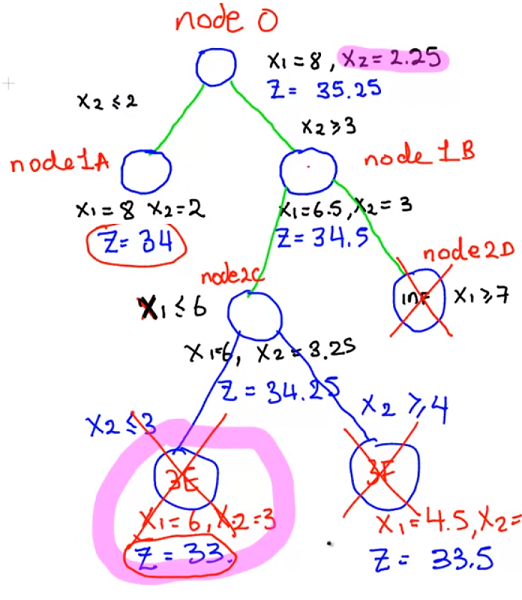
\includegraphics[scale=0.7]{img/branch_and_bound.png}
        \caption{分支定界法例子。}
    \end{center}
\end{figure}
\pagebreak
\begin{enumerate}
    \item 首先考虑 $x_2 \le 2$,也就是 node1A,算得该情况下最优解为 $x_1 = 8, x_2 = 2$,目标函数值为 $34$。这是一个整数解,记录并回溯。
    \item 考虑 $x_2 \ge 3$,也就是 node1B,算得该情况下的最优解为 $x_1 = 6.5, x_2 = 3$,目标函数值为 $34.5$。它还优于我们已知的下界 34,继续搜索。
    \item 考虑 $x_1 \le 6$,也就是 node2C,算得该情况下的最优解为 $x_1 = 6, x_2 = 3.25$,目标函数值为 $34.25$。它还优于我们已知的下界 34,继续搜索。
    \item 考虑 $x_2 \le 3$,也就是 node3E,算得该情况下的最优解为 $x_1 = 6, x_2 = 3$,目标函数值为 $33$。它劣于我们已知的下界 34,回溯。
    \item 考虑 $x_2 \ge 4$,也就是 node3F,算得该情况下的目标函数值为 $33.5$。它劣于我们已知的下界 $34$,回溯。
    \item 考虑 $x_1 \ge 7$,也就是 node2D,该情况下无可行解,回溯。
\end{enumerate}
搜索得最优解为 $x_1 = 8, x_2 = 2$,目标函数值为 $34$。

\pagebreak

\section{贪心算法}
\subsection{一类贪心算法}
\subsubsection{一类贪心算法}
考虑一个有限元素集合 $E$,给 $E$ 中的每个元素 $e$ 定义一个非负的费用 $c(e)$。再考虑 $\mathcal{F} \in 2^E$,对于 $F \in \mathcal{F}$,定义 $F$ 的费用 $c(F) = \sum\limits_{e \in F} c(e)$。一类问题即找出一个 $F$,使得 $c(F)$ 最大(或最小)。

\subsubsection{独立集系统}
对于一个二元组 $(E, \mathcal{F})$,
\begin{enumerate}
    \item $\emptyset \in \mathcal{F}$ 。
    \item $\forall Y \in \mathcal{F}$,$X \subseteq Y \to X \in \mathcal{F}$ 。 
\end{enumerate}
称 $(E, \mathcal{F})$ 为独立系统 (independent system)。 \\
在独立系统 $(E, \mathcal{F})$ 中,$\mathcal{F}$ 中的元素称为独立集,$E - \mathcal{F}$ 中的元素称为相关集。

\subsubsection{基和圈}
将 $\mathcal{F}$ 中的极大独立集称为基 (basis),将 $E - \mathcal{F}$ 中的极小相关集称为圈 (circuit)。
对于 $X \subseteq E$,定义 $X$ 上的基为 $X$ 中的极大独立集。

\subsubsection{秩商}
对于 $X \subseteq E$,$X$ 中的基大小可能不同。定义 $X$ 的秩 $r(X)$ 为 $X$ 中最大的基的大小,类似地定义 $X$ 的下秩 $\rho(X)$ 为 $X$ 中最小的基的大小。
由此定义独立系统的秩商 $q(E, \mathcal{F}) = \min\limits_{x \subseteq E} \quad \frac{\rho(X)}{r(X)}$。秩商是一类问题中贪心解法近似比的下界。

\subsubsection{独立集系统的对偶}
$(E, \mathcal{F}) \rightarrow (E, \mathcal{F}^*)$,$\mathcal{F}^* = \{X \subseteq E \ | \ \exists F$ 的一个基 $\beta, \ X \cap \beta = \emptyset\}$。 \\
有以下性质:
\begin{enumerate}
    \item $(E, \mathcal{F}^*)$是一个独立集系统。
    \item 若$B$是$(E, \mathcal{F})$的基,$E - B$是$(E, \mathcal{F}^*)$的基。
    \item $(E, \mathcal{F}^{**}) = (E, \mathcal{F})$。 \\
    证明:
    \begin{align}
        \nonumber
        \forall X \in \mathcal{F}^{**} & \iff 
        \exists (E, \mathcal{F}^*) \mbox{的一个基}B^*, X \cap B^* = \emptyset \\ & \iff \nonumber
        \exists (E, \mathcal{F}) \mbox{的一个基}B, X \cap (E - B) = \emptyset \\ & \iff \nonumber
        \exists (E, \mathcal{F}) \mbox{的一个基}B, X \subseteq B \\ & \iff \nonumber
        X \subseteq \mathcal{F} \nonumber
    \end{align}
\end{enumerate}

\subsection{一类最大(小)化问题}
根据独立系统的定义,可以引出一类最大(小)化问题。
\begin{itemize}
    \item 最大化问题:给出一个独立系统 $(E, \mathcal{F})$,找出一个 $F \in \mathcal{F}$,使得 $c(F)$ 最大。
    由于每个元素的费用都是非负的,所以 $|F|$ 越大,$c(F)$ 也越大,因此最优的 $F$ 一定是基。
    \item 最小化问题:给出一个独立系统 $(E, \mathcal{F})$,找出一个 $F \in \mathcal{F}$,使得 $F$ 是基,且 $c(F)$ 最小。
\end{itemize}
对任一最大化问题$(E, \mathcal{F})$有$q(E, \mathcal{F}) \le \frac{G(E, \mathcal{F})}{OPT(E, \mathcal{F})} \le 1$,其中$G(E, \mathcal{F})$是贪心算法的目标函数值。 \\
以下证明: \\
$E = \{e_1, \ \cdots, \ e_n\}, \ c: E \rightarrow R^+$。$G_n$是贪心算法的解,$O_n$是最优解,有$G_j = G_n \cap E_j, \ O_j = O_n \cap E_j$,其中$E_j = \{e_1, \ \cdots, \ e_j\}, \ c_1 \le c_2 \le \cdots, c_n, \ G_0 = O_0 = \emptyset$。
\begin{align}
    c(G_n) & = \sum^{n}_{j = 1}(|G_j| - |G_{j - 1}|) \times c_j \tag{1} \\ 
    & = \sum^{n}_{j = 1}|G_j| \times (c_j - c_{j + 1}) \tag{2} \\
    & \ge \sum^{n}_{j = 1}\rho(E_j) \times (c_j - c_{j + 1}) \tag{3} \\ 
    & \ge q\sum^{n}_{j = 1}r(E_j)(c_j - c_{j + 1}) \tag{4} \\
    & \ge q\sum^{n}_{j = 1}|O_j|(c_j - c_{j + 1}) \tag{5} \\ 
    & = q \times c(O_n) \tag{6} \\
    & \Rightarrow \quad \frac{c(G_n)}{c(O_n)} \ge q \tag{7}
\end{align}
($(2) \Rightarrow (3)$:因为$|G_j|$是$E_j$的一个最大独立集;$(4) \Rightarrow (5)$:因为$r(E_j)$是最大个数) \\
$\exists F, \ \frac{\rho(F)}{r(F)} = q(E, F) = \frac{|X|}{|Y|}$, 构造
$$
c(e) = 
\begin{cases}
1, \ e \in F \\
0, \ e \notin F
\end{cases} \\
(c_1 = c_2 = \cdots = c_{|X|} = 1, \ c_{|X| + 1} = \cdots = c_n = 0)
$$

\subsubsection{最大化问题的实例}
\begin{itemize}
    \item $0-1$ 背包问题:$E$ 中的元素是每个物品,$\mathcal{F}$ 中的元素是所有可以放进背包的物品集合,费用就是物品的价值。
    \item 最大权独立集:$E$ 中的元素是点,$\mathcal{F}$ 中的元素是独立集,费用就是每个点的权值。
    \item 最长简单路径:$E$ 中的元素是边,$\mathcal{F}$ 中的元素是所有从起点到终点的简单路径以及其子集,费用就是每条边的距离。
    \item 最大权森林:$E$ 中的元素是边,$\mathcal{F}$ 中的元素是所有不含圈的边集,费用就是每条边的权值。
\end{itemize}

\subsubsection{最小化问题的实例}
\begin{itemize}
    \item 最小生成树问题:$E$ 中的元素是边,$\mathcal{F}$ 中的元素是所有不含圈的边集,费用就是每条边的权值。
    \item 最短路问题:$E$ 中的元素是边,$\mathcal{F}$ 中的元素是所有从起点到终点的简单路径以及其子集,费用就是每条边的距离。
    \item 旅行商问题:$E$ 中的元素是边,$\mathcal{F}$ 中的元素是哈密尔顿回路及其子集,费用就是每条边的距离。
\end{itemize}

\subsection{拟阵}
拟阵 (matroid)是一个特殊的独立集系统。一个独立系统需要满足以下三个条件中的一个才被称为是拟阵(以下三个条件等价):
\begin{enumerate}
    \item 若 $X, Y \in \mathcal{F}$,且 $|X| > |Y|$,则 $\exists e \in X - Y$,$Y \cup \{e\} \in \mathcal{F}$。
    \item 若 $X, Y \in \mathcal{F}$,且 $|X| = |Y| + 1$,则 $\exists e \in X - Y$,$Y \cup \{e\} \in \mathcal{F}$。
    \item $\forall X \subseteq E$,$X$ 的所有基大小相同。
\end{enumerate}

\subsubsection{例子}
\begin{enumerate}
    \item $E = \{v_1, \ \cdots, \ v_m\}$,$\mathcal{F} = \{z \subseteq E \ | \ z$是线性无关组$\}$。
    \item $E$是有限集合,$\mathcal{F} = \{X \subseteq E, |X| \le k \in N\}$。(一致拟阵)
    \item $E$是无向图$G$,$\mathcal{F} = \{X \subseteq E, X$构成一个森林$\}$。(图拟阵)
\end{enumerate}

\subsubsection{拟阵的交}
假设有两拟阵$(E, \mathcal{F}_1)$,$(E, \mathcal{F}_2)$,其交为$(E, \mathcal{F}_1 \cap \mathcal{F}_2)$。 \\
$n$ 个拟阵的交,用贪心算法得到的解近似比为 $\frac{1}{n}$。 \\~\\
任一个独立集系统都是有限个拟阵的交。 \\
以下证明: \\
独立集系统$(E, \mathcal{F})$,假设其有$k$个圈$C_1, \ \cdots, C_k$,$F_i = \{X \subseteq E | X \nsupseteq C_i\}$。 \\
$(E, \mathcal{F}_i), \ \forall \mathcal{F} \subseteq E$,此时有两种可能:
\begin{enumerate}
    \item $F \nsupseteq C_i$。
    \item $F \supseteq C_i$,$\forall e \in C_i, \mathcal{F} - \{e\}$是极大独立集。
\end{enumerate}
$\forall X \in \mathcal{F}, X$不含任何圈$\iff X \in \cap^{k}_{i = 1}\mathcal{F}_i$ \\
$(E, \mathcal{F})$为独立集系统,$\mathcal{F} = \cap^{k}_{i = 1}\mathcal{F}_i$。 \\
设$F \subseteq E$,考虑$(E, \mathcal{F})$在$\mathcal{F}$上,两个不同的极大独立集,$A, B \ (|B| \ge |A|)$欲证$|B| \le k|A|$。 \\
$\forall e \in B - A$,有$e \notin \cap^{k}_{i = 1} (A_i - A)$,$A_i: (E, \mathcal{F}_i)$在$A \cup B$含$A$极大独立集,则$e$最多出现在$(k - 1)$个$A_i - A$中,$\sum^{k}_{i = 1}|A_i - A| \le (k - 1)|B - A| \le (k - 1)|B|$,
同理$k|B| \le \sum^{k}_{i = 1}|A_i| $(因为极大独立集有相同维数)$\le k|A| + (k - 1)|B|$。 \\
得证$|B| \le k|A|$。

\subsection{两类贪心算法}
\subsubsection{Best in}
将 $E$ 中所有元素按费用从大到小排序,使得 $c(e_1) \ge c(e_2) \ge ... \ge c(e_n)$。假设 $F = \emptyset$,依照 $e_1, e_2 \dots, e_n$ 的顺序考虑,若 $e_i$ 加入 $F$ 后 $F$ 仍是独立集,就加入$e_i$。此贪心算法用于解决最大化问题。 \\
设 $G(E, \mathcal{F})$ 表示 Best in 算法得到的解;$\text{OPT}(E, \mathcal{F})$ 表示最优解,则 $$q(E, \mathcal{F}) \le \frac{G(E, \mathcal{F})}{\text{OPT}(E, \mathcal{F})} \le 1$$ 从此定理可以看出:若一个独立集系统是拟阵,则用 Best in 算法得到的最大化问题的解一定是最优解。

\subsubsection{Worst out}
将 $E$ 中所有元素按费用从大到小排序,使得 $c(e_1) \ge c(e_2) \ge ... \ge c(e_n)$。假设 $F = E$,依照 $e_1, e_2 \dots, e_n$ 的顺序考虑,若把 $e_i$ 从 $F$ 中去掉后 $F$ 还含有至少一个基,就去掉$e_i$。此贪心算法用于解决最小化问题。 \\
使用 Worst out 贪心得到的解满足 
$$
1 \le \frac{G(E, \mathcal{F})}{\text{OPT}(E, \mathcal{F})} \le \max\limits_{F \subseteq E} \quad \frac{|F| - \rho^*(F)}{|F| - r^*(F)}
$$ 
其中 $\rho^*(F)$ 表示对偶独立集系统中的下秩,$r^*(F)$ 表示对偶独立系统中的秩。

\pagebreak

\section{近似算法}
\subsection{近似算法}
算法$A$是一近似算法 (approximation),$A(I)$是算法$A$在例子$I$的目标函数值,$OPT(I)$是最优解的目标函数值。 \\
算法$A$的近似比$\rho_A = \sup_{I}\{\frac{OPT(I)}{A(I)}, \frac{A(I)}{OPT(I)}\}$。
称算法$A$为$r$近似,在极大化问题中,$\forall I, OPT(I) \le r \times A(I)$;或在极小化问题中,$\forall I, A(I) \le r \times OPT(I)$。

\subsection{背包问题}
假设$s_i$表示物品$i$的所占空间,$v_i$表示物品$i$的价值,$C$表示总共空间,$F_j(i)$表示前$j$个物品中价值和为$i$的物品所需最小空间,有
$$
OPT: argmax \{i | F_j(i) \le c\},F_j(i) = min\{F_{j - 1}(i), F_{j - 1}(i - v_i) + s_i\}
$$
时间复杂度为$O(n^2v_{max})$属于伪多项式时间算法。 \\
若将各个物品的价值缩小$K$倍,$v_i' =  \left\lfloor\frac{v_i}{K}\right\rfloor $,此时时间复杂度变为$O(\frac{n^2v_{max}}{K})$。 \\
令动态规划的解为$S'$,原问题最优解为$S^*$,有
\begin{align}
    \sum_{j \in S'}v_j & \ge \sum_{j \in S'}\left\lfloor\frac{v_j}{K}\right\rfloor \times K \nonumber \\
    & = K \times \sum_{j \in S'}v_j' \nonumber \\
    & \ge K \times \sum_{j \in S^*}v_j'\nonumber \\
    & \ge \sum_{j \in S^*}(\frac{v_j}{K} - 1) \times K \nonumber \\
    & = \sum_{j \in S^*}v_j - K|S^*| \nonumber \\
    & \ge OPT - n \times K \nonumber
\end{align}
希望
\begin{align}
    n \times K &\le \epsilon \times OPT \nonumber \\ 
    & \Rightarrow K \le \frac{\epsilon}{n} \times v_{max} \ \mbox{(因为}OPT \ge v_{max}\mbox{)} \nonumber \\
    & \mbox{(令} K = \frac{\epsilon}{n} \times v_{max} \mbox{)} \nonumber \\
    & \Rightarrow OPT - n \times K = (1 - \epsilon) \times K \nonumber
\end{align}
% 令$K = \frac{\epsilon}{n} \times v_{max}$,$OPT - n \times K = (1 - \epsilon) \times K$,
此时时间复杂度变为$O(\frac{n^2v_{max}}{K}) = O(\frac{n^3}{\epsilon})$。

\subsection{顶点覆盖}
\subsubsection{近似算法$1$}
假设共有 $n$ 个点,$x_i$ 表示第 $i$ 个点是否在答案集合中,$w_i$ 表示第 $i$ 个点的权重,$E$ 表示边集,$(u, v)$ 表示连接点 $u$ 与点 $v$ 的一条边。构造出顶点覆盖 (vertex cover) 模型:
$$
\min \quad \sum_{i = 1}^n w_ix_i
$$
$$
\text{s.t.} 
\begin{cases}
    x_i + x_j \ge 1, \ \forall (i, j) \in E \\
    x \in \{0, 1\}
\end{cases}
$$
这是一个整数规划问题,假设该问题的最优目标函数值为 $\text{OPT}$。 \\
对该问题进行松弛,将 $x \in \{0, 1\}$ 改为 $x \ge 0$。设松弛后的线性规划问题最优解为 $x^*$,最优目标函数值为 $\text{OPT}_{LP}$,有 $\text{OPT}_{LP} \le \text{OPT}$。
构造出原问题的可行解 $x$ 如下:
$$
x_i = \begin{cases} 1 & x^*_i \ge 0.5 \\ 0 & x^*_i < 0.5 \end{cases}
$$ 
由于对于每条边 $(i, j)$ 存在 $x^*_i + x^*_j \ge 1$ 的限制,则 $\max(x^*_i, x^*_j) \ge 0.5$,$x_i + x_j \ge 1$ 仍然成立,此解可行。 \\
有 $x_i \le 2x^*_i$。将构造的可行解代入目标函数,有
$$
\sum_{i=1}^n w_ix_i \le 2\sum_{i=1}^n w_ix^*_i \le 2\text{OPT}_{LP} \le 2\text{OPT}
$$
证明了算法的近似比为 $2$。

\subsubsection{近似算法$2$:原始对偶算法}
有对偶问题:
$$
\max \quad \sum_{e \in E} y_e
$$
$$
\text{s.t.} 
\begin{cases}
    \sum_{i \in e} y_e \le w_i, \ \forall i \in V \\
    y_e \ge 0
\end{cases}
$$
互补松弛条件:
\begin{itemize}
    \item PCS(原始问题的互补松弛条件):$x_i \times (w_i - \sum_{i \in e}y_e) = 0$。
    \item DCS(对偶问题的互补松弛条件):$y_e \times (x_i + x_j - 1) = 0$。
\end{itemize}
若PCS成立,有
$$
\begin{cases}
x_i \ne 0 \Rightarrow w_i = \sum_{i \in e}y_e \\
y_e \ne 0 \Rightarrow 1 \le x_i + x_j \le 2
\end{cases}
$$
则
\begin{align}
    \sum_{i = 1}^nw_ix_i & = \sum_{i = 1}^n (\sum_{i \in e}y_e)x_i \nonumber \\ 
    & \le 2 \times \sum_{e \in E}y_e \nonumber \\
    & \le 2 \times \sum_{i = 1}^n w_ix_i^* \nonumber \\ 
    & \le 2 \times C_{IP}^* \nonumber
\end{align}
算法步骤:
\begin{enumerate}
    \item $x = 0, y = 0$,所有边未标记。
    \item 任选一条未标记的边,提升$y_e$到其某一端点约束变紧。
    \item $x_i = 1$,与$v_i$关联的边全部标记。
    \item 重复上述第二、第三步骤,直到所有边被标记。
\end{enumerate}
假设有以下问题:
\begin{figure}[H]
    \begin{center}
        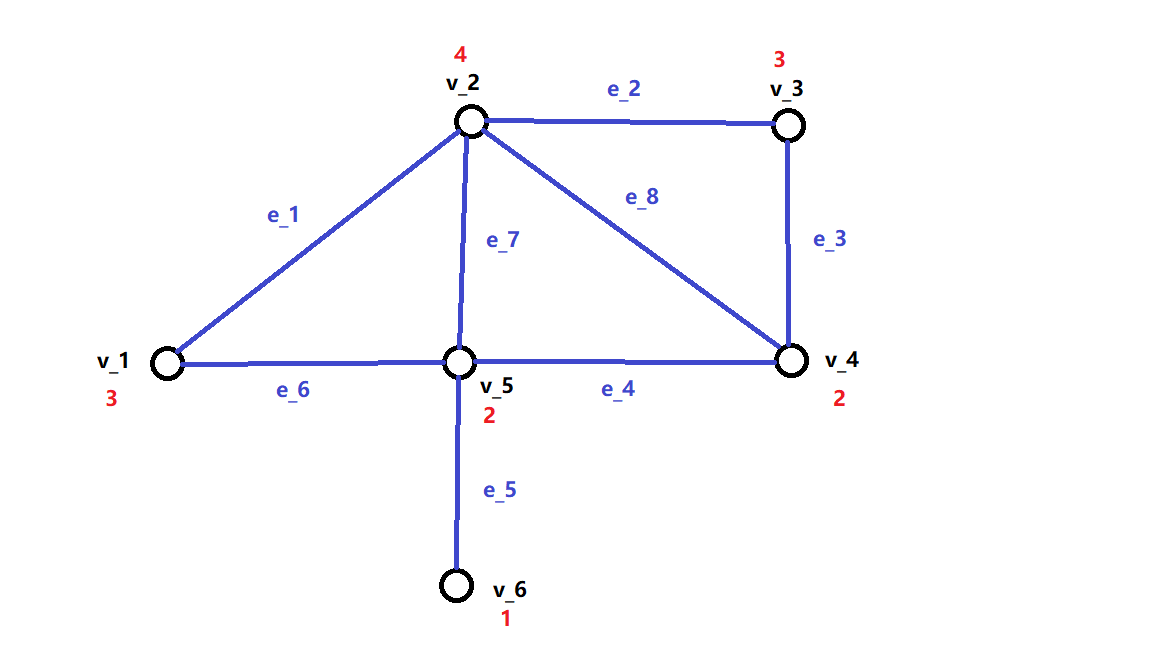
\includegraphics[scale=0.4]{img/vertex_cover.png}
        \caption{顶底覆盖例子。}
    \end{center}
\end{figure}
\begin{enumerate}
    \item 先选$v_1$,提升$e_1 = 3$,$v_1$覆盖,因为$e_6$连接$v_5$,提升$e_6 = 3 - 3 = 0$。
    \item 选择$v_2$,提升$e_2 = 4 - 3 = 1$,$v_2$覆盖,因为$e_7$连接$v_5$,提升$e_7 = 4 - 3 - 1 = 0$;$e_8$连接$v_4$,提升$e_8 =  4 - 3 - 1 - 0 = 0$。
    \item 选择$v_3$,提升$e_3 = 3 - 1 = 2$,$v_3$覆盖。
    \item 选择$v_4$,提升$e_4 = 2 - 0 - 2 = 0$,$v_4$覆盖。
    \item 选择$v_6$,提升$e_5 = 1$,$v_6$覆盖。
\end{enumerate}
得到原问题权重:$13$(点);对偶问题权重:$7$(边)。
\begin{figure}[H]
    \begin{center}
        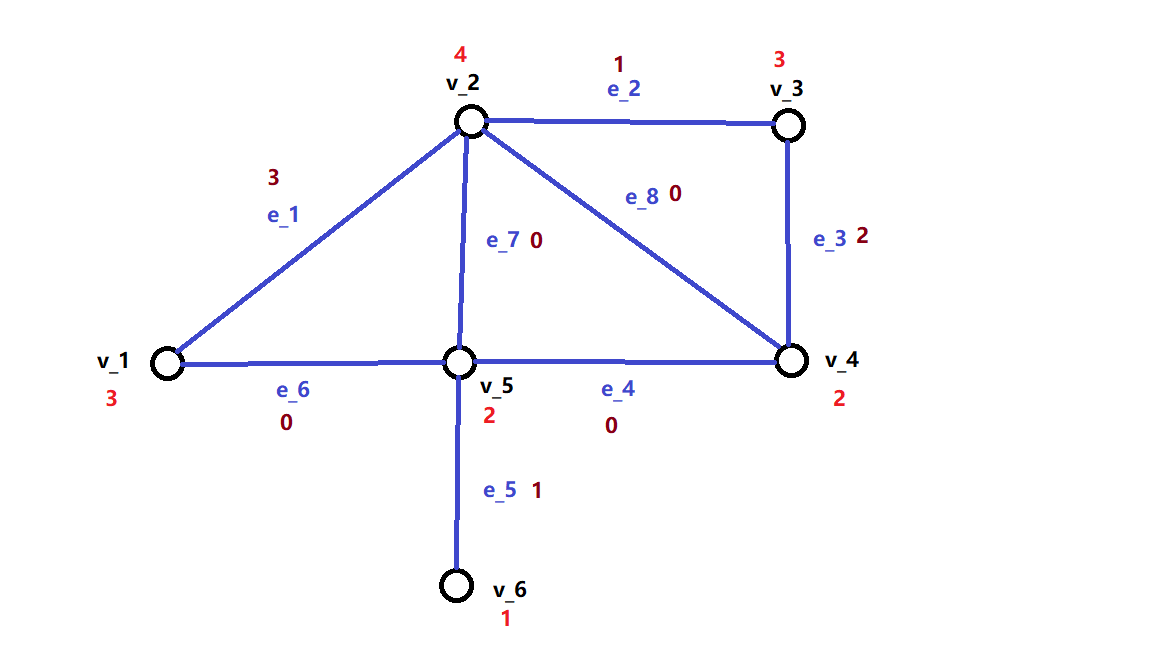
\includegraphics[scale=0.5]{img/vertex_cover_result.png}
        \caption{顶底覆盖例子结果。}
    \end{center}
\end{figure}

\subsection{非等同并行机调度}
有 $m$ 台机器和 $n$ 件物品,每件物品都要在一台机器上加工,$a_{i, j}$表示第 $i$ 台机器加工第 $j$ 件物品的时间。求一种把物品分配给机器的方案,使得加工总时长最长的机器,加工总时长最短,即为非等同并行机调度 (Unrelated Parallel Machine Scheduling, UPMS)。
构造出模型:
$$
\min \quad T
$$
$$
\text{s.t.} 
\begin{cases}
    \sum_{i = 1}^m x_{i, j} = 1, \ \forall j \in \{1, 2, \ \cdots, n\} \\
    \sum_{j = 1}^n a_{i, j}x_{i, j} \le T, \ \forall i \in \{1, 2, \ \cdots, m\} \\
    x_{i, j} \in \{0, 1\}
\end{cases}
$$
此模型不适合进行松弛。假设只有一件物品需要加工,且该物品在所有机器上的加工时间都为 $1$,则原问题的最优目标函数值为 $1$,然而松弛求出的最优解为 $x_{i, 1} = 1/m$,下界不够紧,难以进行近似比分析。 \\~\\
先二分 $T$ 。若 $a_{i, j} > T$,加上 $x_{i, j} = 0$ 的限制,让改动后的问题存在可行解的最小的 $T$,就是原问题最优目标函数值的下界(可利用两阶段法的第一阶段判断是否存在可行解)。 \\
假设改动后的问题最优解为 $x^*$,对于第 $j$ 件物品,若 $\exists i, x^*_{i, j} = 1$ ,则称该物品为“整数物品”,否则称该物品为“分数物品”,假设共有 $n_1$ 个“整数物品”, $n_2$ 个“分数物品”。有 $n_1 + n_2 = n$, 若第 $j$ 件物品为“分数物品”, $x_{i, j}$ 中至少有两个非零值。
由于原问题有 $n + m$ 条限制,根据单纯形法,非零的变量至多有 $n + m$ 个,有 $n_1 + 2n_2 \le n + m$,得到 $n_2 \le m$。 \\~\\
通过使得每台机器的加工总时长都不超过 $2T$,设计一个近似比为 $2$ 的算法。 \\
定义:若连通图中边数小等于点数,称该连通图为伪树;若一张图的所有连通块都是伪树,称该图为伪森林。 \\
构造一张二分图:左边有 $m$ 个点,每个点表示一台机器;右边有 $n$ 个点,每个点表示一件物品。若 $x_{i, j} > 0$ 则连接第 $i$ 台机器和第 $j$ 件物品。如果这个二分图不连通,那么对每个连通块分别求解,最后将解合并即为答案,因此可以假设该二分图连通。由于非零变量至多有 $n+m$ 个,所以该连通图的边数不超过点数,是一个伪树。 
首先考虑“整数物品”。每个“整数物品” $j$ 都只和一台机器 $i$ 有连边 $(i, j)$,将“整数物品” $j$ 放在机器 $i$ 中加工,并去掉物品 $j$ 和边 $(i, j)$。由于每次恰好去除一个点和一条边,这张图仍然是伪树。此时每台机器的加工总时长至多为 $T$,否则问题的最优目标函数值就会超过 $T$ 。 \\
此时,仅剩机器和“分数物品”了。考虑所有度数为 $1$ 的机器 $i$。假设唯一连接机器 $i$ 的边是 $(i, j)$,将“分数物品” $j$ 放在机器 $i$ 中加工,并去掉机器 $i$、物品 $j$ 和物品 $j$ 的所有连边。由于每件“分数物品”都有至少两条连边,所以我们每次都会去掉两个点以及至少两条边,可知剩下的图是伪森林。
反复删除度数为 $1$ 的机器,直到最后不存在度数为 $1$ 的机器为止。 \\
由于剩下的图是伪森林也是二分图,则剩下的图中只能包含若干偶环,在偶环上任意给每台机器分配一件物品即可。 \\
因此,每台机器至多分配到一个“分数物品”,再加上原来分配给它的“整数物品”,每台机器的总加工时长至多为 $2T$,得到一个近似比为 $2$ 的算法。

\subsection{装箱问题}
\subsubsection{均摊体积}
假设第 $i$ 件物品体积为 $a_i$,定义权重 $w(a_i)$ :
$$
w(a_i) = \frac{6}{5}a_i + v(a_i)
$$
称 $v$ 为 bonus,定义为:
$$
v(a_i) = \begin{cases} 0 & a_i \le \frac{1}{6} \\ \frac{3}{5}(a_i - \frac{1}{6}) & \frac{1}{6} < a_i \le \frac{1}{3} \\ \frac{1}{10} & \frac{1}{3} < a_i \le \frac{1}{2} \\ \frac{2}{5} & a_i > \frac{1}{2} \end{cases}
$$
记 $w(I)$ 为装箱问题 (bin packing)的一个实例 $I$ 的权重总和,$\text{FF}(I)$ 表示对实例 $I$ 运用 First fit 算法得到的目标函数值,$\text{OPT}(I)$ 表示实例 $I$ 的最优目标函数值。
再记 $B$ 为 first fit 算法得到的方案,$B^*$ 为最优方案,$c(B_j)$ 表示第 $j$ 个 bin 中物品的体积总和,$w(B_j)$ 表示第 $j$ 个 bin 中物品的权重总和,有
$$
w(I) = \sum\limits_{i=1}^n w(a_i) = \sum\limits_{j=1}^{\text{FF}(I)}w(B_j) = \sum\limits_{j=1}^{\text{OPT}(I)}w(B^*_j)
$$
先是证明均摊体积不超过$1.7$。 \\
对于一个箱子,可分以下情况讨论:
\begin{enumerate}
    \item 所有物品体积 $c$ 均有 $c \le \frac{1}{6}$。箱子的权重就是箱中物品体积总和的 $1.2$ 倍,不会超过 $1.7$。
    \item 存在物品体积 $c$ 有 $\frac{1}{6} < c \le \frac{1}{2}$。这种物品在一个箱中至多有 $5$ 个,bonus 不会超过 $\frac{1}{10} \times 5 = \frac{1}{2}$,权重也不会超过 $1.7$。
    \item 存在两个物品体积 $c_1$ 和 $c_2$ 有 $c_1 > \frac{1}{2}$ 且 $\frac{1}{3} < c_2 \le \frac{1}{2}$。其它物品的体积都不会超过 $\frac{1}{6}$,没有 bonus;$c_1$ 和 $c_2$ 带来的 bonus 恰为 $0.5$,权重不会超过 $1.7$。
    \item 存在三个物品体积 $c_1$,$c_2$ 和 $c_3$ 有 $c_1 > \frac{1}{2}$,$\frac{1}{6} < c_2, c_3 \le \frac{1}{3}$ 且 $c_2 + c_3 < \frac{1}{2}$。其它物品的体积都不会超过 $\frac{1}{6}$,没有 bonus;$c_2$ 和 $c_3$ 带来的 bonus 为 $\frac{3}{5}(c_2 - \frac{1}{6}) + \frac{3}{5}(c_3 - \frac{1}{6}) < 0.1$,再加上 $c_1$ 带来的 bonus $0.4$,权重不会超过 $1.7$。
\end{enumerate}
证明了均摊体积不超过$1.7$。 \\~\\
接着证明除两个箱子外,其它箱子的权值均值至少为$1$。
首先去掉权值至少为 $1$ 的箱子,考虑权值不足 $1$ 的箱子。可知权值不足 $1$ 的箱子有以下性质:
\begin{enumerate}
    \item 不含体积至少为 $0.5$ 的物品,因为若含体积大于$0.5$的物品,该物品的权重就会超过$1$。
    \item 一个箱中不会包含两个体积至少为 $\frac{1}{3}$ 的物品,因为若含两个体积大于$\frac{1}{3}$的物品,该两个物品的权重就会超过$1$。
    \item 箱子的体积之和小于 $\frac{5}{6}$,因为若箱子的体积之和大于$\frac{5}{6}$,不算bonus就足以使权重超过$1$。
\end{enumerate}
可得
\begin{enumerate}
    \item 除了最后一个箱子,其它箱子中至少有两个物品。
    \item 除了最后两个箱子,其它箱子的体积之和都大于 $\frac{2}{3}$(如果有一个 bin 的体积之和不超过 $\frac{2}{3}$,由于是 First fit 算法,后面的箱子里的物品体积至少为 $\frac{1}{3}$ 但少于 $\frac{1}{2}$;而后面至少还有两个箱子,违反了“一个箱子内不会包含两个体积至少为 $\frac{1}{3}$ 的物品”的性质)。
\end{enumerate}
再来证明一个引理:如果两个箱子 $B_1$ 和 $B_2$ 满足 $B_1$ 在 $B_2$ 前面、$w(B_1), w(B_2) < 1$、$c(B_1) \ge \frac{2}{3}$ 以及 $B_2$ 有至少两个物品,则 $\frac{6}{5}c(B_1) + v(B_2) \ge 1$。 \\
有以下性质:
\begin{enumerate}
    \item $c' \ge \frac{1}{6}$,否则 $B_1$ 将会与“箱子的体积之和小于 $\frac{5}{6}$”的性质矛盾。
    \item $ c' < \frac{1}{3}$,否则 $B_2$ 将会与“一个箱子中不会包含两个体积至少为 $\frac{1}{3}$ 的物品”的性质矛盾。
    \item $c' > 1 - c(B_1)$,否则 $c'$ 就会放进 $B_1$ 。
\end{enumerate}
得到 $\frac{1}{6} \le c' < \frac{1}{3}$,则
\begin{align}
    \frac{6}{5}c(B_1) + v(B_2) & \ge \frac{6}{5}c(B_1) + 2 \times v(c') \nonumber \\ 
    & > \frac{6}{5}c(B_1) + \frac{6}{5}(1 - c(B_1) - \frac{1}{6}) \nonumber \\ 
    & = 1 \nonumber
\end{align}
假设 First fit 算法得到的方案中,权重之和小于 $1$ 的箱子按先后顺序为 $B_1, B_2, \dots, B_k$,则
\begin{equation}
\begin{split}
    & w(B_1) + w(B_2) + \dots + w(B_{k-2}) + w(B_{k-1}) + w(B_k) \nonumber \\ 
    = & \ v(B_1) + (\frac{6}{5}c(B_1) + v(B_2)) + \dots + (\frac{6}{5}c(B_{k-2}) + v(B_{k-1})) \nonumber \\
    + & \ (\frac{6}{5}c(B_{k-1}) + \frac{6}{5}c(B_k)) + v(B_k) \nonumber \\ 
    \ge & \ (k-2) + \frac{6}{5} \nonumber
\end{split}
\end{equation}
即除了最后两个箱子,其它的箱子权值均值都至少为$1$,再加上$0.8$以及权值至少为 $1$ 的箱子,则所有的箱子的权值均值就都至少为 $1$。证明First fit算法有 $1.7$ 的近似比。

\subsection{旅行商问题}
在满足三角不等式的完全图上,旅行商问题 (Travelling Salesman Problem, TSP),可通过搜索最小生成树 (Minimum Spanning Tree, MST),将树上每条边重复一次变成欧拉图 (Euler graph),在欧拉图上 short-cutting,得到近似比为 $2$的上界。 \\
下面证明近似比为$1.5$的近似算法: \\
将树上度数为奇数的点进行配对(一张图上度数为奇数的点有偶数个),每一对之间连一条边,则构成的图上的点的度数都是偶数,即为欧拉图。 \\
\begin{figure}[H]
    \begin{center}
        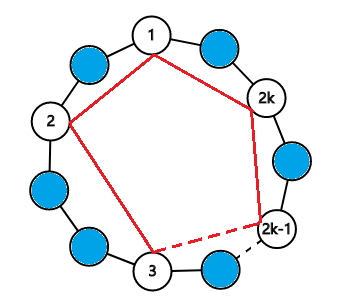
\includegraphics[scale=0.8]{img/tsp.png}
        \caption{度数为奇数的点匹配示意图。}
        \label{img:tsp}
    \end{center}
\end{figure}
在图\ref{img:tsp} 上,白色的点是最小生成树上的度数为奇数的点。将奇点按顺序进行 short-cutting,得到两个不相交匹配($1 - 2, 3 - 4, \cdots, (2k - 1) - 2k$ 以及 $2 - 3, 4 - 5, \cdots, 2k - 1$)。由于满足三角不等式,这两个匹配的权值之和不大于 $\text{OPT}$,则两个匹配中较小的权值不大于 $0.5\text{OPT}$。因为算法中求出的是最小完美匹配,则最小完美匹配的权值也不大于 $0.5\text{OPT}$。
因此,最小生成树和最小权完美匹配证明了 $1.5$ 的近似比。
\begin{figure}[H]
    \begin{center}
        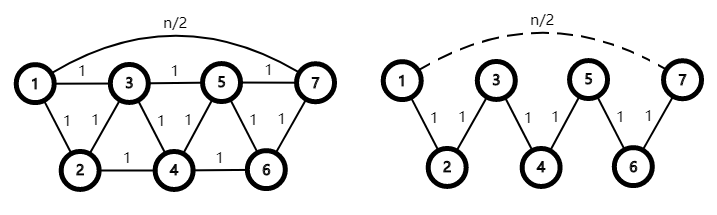
\includegraphics[scale=0.8]{img/tsp_2.png}
        \caption{最小权完美匹配示意图。}
        \label{img:tsp_2}
    \end{center}
\end{figure}
图\ref{img:tsp_2} 可说明近似比$1.5$是紧的。途中没有画出来的边权值都是 $2$,右图实线是算法可能获得的最小生成树,虚线是算法可能算出的最小权完美匹配。可得最优解为 $n$,而算法可能得出的解是 $n + \frac{n}{2}$。 \\
只要“梯形”上面的点足够多,则近似比为 $1.5$。

\subsubsection{满足三角不等式的完全图的最短哈密尔顿路}
在满足三角不等式的完全图中,求最短哈密尔顿路 (shortest Hamiltonian path)。
算法步骤:
\begin{enumerate}
    \item 求个最小生成树 $T$。假设$S$为在最小生成树上度数为奇数的点的集合。
    \item 求 $S$ 的最小权匹配 $M$。假设最优解上有 $2t$ 个度数为奇数的点,则可以拆成两个匹配:$1 - 2, 3 - 4, \cdots, (2t - 3) - (2t - 2)$($(2t - 1)$ 和 $2t$ 没有匹配) 与 $2 - 3, 4 - 5, 6 - 7, \cdots, (2t - 2) - (2t - 1)$($1$ 和 $2t$ 没有匹配,其中$u - v$表示点$u$和点$v$匹配),可以证明 $M$ 的权值之和至多为 $0.5\text{OPT}$。
    \item $T \cup M$ 即为一张有欧拉路 (Euler path)的图,通过 short-cutting 把欧拉路变成哈密尔顿路即可。
\end{enumerate}
此算法的近似比为$1.5$。

\subsubsection{与哈密尔顿圈相关的优化问题}
\begin{itemize}
    \item 最长哈密尔顿路 (Longest Hamiltonian path)。
    \item 最小圈覆盖 (Minimum cycle cover problem, MCCP).
    \item 最小双联通子图 (Minimum biconnected subgraph(边数最少)).
    \item 最小分支双联通子图 (Minimum branch biconnected subgraph).
    \item 最大内部生成树 (Maximum internal spanning tree(叶子节点最少)).
\end{itemize}

\pagebreak

	\chapter{Convex Optimization}
\section{Convex Functions}
Definitions: 
\begin{itemize}
    \item Convex set: contains the line through any two distinct points in the set. $x_1, x_2 \in \mathbb{C}, 0 \le \theta \le 1 \Rightarrow \theta x_1 + (1 - \theta)x_2 \in \mathbb{C}$. Intersection of convex sets is convex.
    \item Convex combination of $x_1, x_2, \cdots, x_n$: any point $x$ of the form $x = \theta_1x_1 + \theta_2x_2 + \cdots + \theta_kx_k$, where $\theta_1 + \theta_2 + \cdots + \theta_k = 1, \theta_i \ge 0$.
    \item $f: \mathbb{R}^n \rightarrow \mathbb{R}$ is convex if $\text{dom} f$ is a convex set and 
    $$
    f(\theta x + (1 - \theta)y) \le \theta f(x) + (1 - \theta)f(y), \ \forall x, y \in \text{dom} f, 0 \le \theta \le 1
    $$
    $f$ is concave if $-f$ is convex.
    \item Sublevel set: $\alpha$-sublevel set of $f: \mathbb{R}^n \rightarrow \mathbb{R}$:
    $$
    C_{\alpha} = \{x \in \text{dom} f | f(x) \le \alpha\}
    $$
    Sublevel sets of convex functions are convex.
    \item Epigraph of $f: \mathbb{R}^n \rightarrow \mathbb{R}$: 
    $$
    epi \ f = \{(x, t) \in \mathbb{R}^{n + 1} | x \in \text{dom} f, \ f(x) \le t\}
    $$
    $f$ is convex if and only if $epi \ f$ is a convex set.
\end{itemize}
\subsection{First-order condition}
$f$ is differentiable if $\text{dom} f$ is open and the gradient
$$
\nabla f(x) = (\frac{\partial f(x)}{\partial x_1}, \frac{\partial f(x)}{\partial x_2}, \cdots, \frac{\partial f(x)}{\partial x_n}), \ \forall x \in \text{dom} f
$$
Differentiable $f$ with convex domain is convex if and only if 
$$
f(y) \ge f(x) + \nabla f(x)^T(y - x)
$$

\subsection{Second-order condition}
$f$ is twice differentiable if $\text{dom} f$ is open and the Hessian $\nabla^2 f(x) \in \mathbb{S}^n$
$$
\nabla^2 f(x)_{ij} = \frac{\partial^2 f(x)}{\partial x_i \partial y_j'}, \ \forall i, j = 1, 2, \cdots, n, \ x \in \text{dom} f
$$
Twice differentiable $f$ with convex domain is convex if and only if $\nabla^2 f(x) \succcurlyeq 0, \ \forall x \in \text{dom} f$. And if $\nabla^2 f(x) \succ 0, \ \forall x \in \text{dom} f$, then $f$ is strictly convex.

\subsection{Examples of convex and concave functions}
\begin{itemize}
    \item Convex.
    \begin{itemize}
        \item Affine: $ax + b, \ \forall a, b \in \mathbb{R}$.
        \item Exponential: $e^{ax}, \ \forall a \in \mathbb{R}$.
        \item Powers: $x^a, \ \forall a \ge 0 \ or \ a \le 0$.
        \item Negative entropy: $x\log x \ on \ \mathbb{R}_{++}$.
        \item All Norms: $||x||_p$.
    \end{itemize}
    \item Concave.
    \begin{itemize}
        \item Affine: $ax + b, \ \forall a, b \in \mathbb{R}$.
        \item Powers: $x^a, \forall 0 \le a \le 1$.
        \item Negative entropy: $x\log x \ on \ \mathbb{R}_{++}$.
    \end{itemize}
\end{itemize}

\subsection{Operations that preserve convexity}
\begin{itemize}
    \item Positive weighted sum and composition with affine function
    \begin{itemize}
        \item Nonnegative multiple: $\alpha f$ is convex if $f$ is convex and $\alpha \ge 0$.
        \item Sum: $f_1 + f_2$ is convex if $f_1, f_2$ are convex.
        \item Composition with affine function: $f(Ax + b)$ is convex if $g$ is convex.
    \end{itemize}
    \item Pointwise maximum: If $f_1, f_2, \cdots, f_m$ are convex, then $f(x) = \max\{f_1(x), \cdots, f_m(x)\}$ is convex.
    \item Pointwise supermum: If $f(x, y$) is convex in $x$ for each $y \in \mathcal{A}$, then $g(x) = \sup_{u \in \mathcal{A}} f(x, y)$ is convex.
    \item Composition with scalar functions: $g: \mathbb{R}^n \rightarrow \mathbb{R}$, $h: \mathbb{R} \rightarrow \mathbb{R}$ and $f(x) = h(g(x))$. $f$ is convex if 
    \begin{itemize}
        \item $g$ and $f$ are convex and $\tilde{h}$ is nondecreasing.
        \item $g$ is concave, $h$ is convex and $\tilde{h}$ is nonincreasing.
    \end{itemize}
    \item Minimization: If $f(x, y)$ is convex in $(x, y)$ and $C$ is a convex set, then $g(X) = \inf_{y \in C} f(x, y)$ is convex. Distance to a set: $dist(x, S) = \inf_{y \in S} ||x - y||$ is convex if $S$ is convex.
    \item Perspective: The perspectiveof a function $f: \mathbb{R}^n \rightarrow \mathbb{R}$ is the function $g:\mathbb{R}^n \times \mathbb{R} \rightarrow \mathbb{R}$.
    $$
    g(x, t) = tf(\frac{x}{t}), \ \text{dom} g = \{(x, t) | \frac{x}{t} \in \text{dom} f, t > 0\}
    $$
    $g$ is convex if $f$ is convex.
\end{itemize}
\pagebreak

\section{Convex Optimization Problems}
\subsection{Optimization problem in standard form}
$$
\min \quad f_0(x)
$$
$$
\text{s.t.} 
\begin{cases}
    f_i(x) \le 0, \ \forall i = 1, 2, \cdots, m \\
    h_i(x) = 0, \ \forall i = 1, 2, \cdots, p \\
\end{cases}
$$
\begin{itemize}
    \item $f_i: \mathbb{R}^n \rightarrow \mathbb{R}$: are inequality constraint functions.
    \item $h_i: \mathbb{R}^n \rightarrow \mathbb{R}$: are equality constraint functions.
    \item Optimal value: 
    $$
    p^* = inf\{f_0(x) | f_i(x) \le 0, \ \forall i = 1, 2, \cdots, m. \ h_i(x) = 0, \ \forall i = 1, 2, \cdots, p\}
    $$
    $p^* = \infty$, if problem is infeasible; $p^* = - \infty$, if problem is unbounded below.
\end{itemize}

\subsection{Local and global optimal}
\begin{itemize}
    \item Any locally optimall point of a convex problem is (globally) optimal. \\
    Proof: \\
    Suppose $x$ is locally optimal and $y$ is optimal with $f_0(y) < f_0(x)$. \\
    $x$ is locally optimal means there is an $R > 0$ such that
    $$
    (z \ is \ feasible) \ ||z - x||_2 \le R \Rightarrow f_0(z) \ge f_0(x)
    $$
    Consider $z = \theta y + (1 - \theta)x$ with $\theta = \frac{R}{2||y - x||_2}$. $||y - x||_2 > R$, so $0 < \theta < 1/2$. \\
    $z$ is a convex combination of two feasible points, and $||z - x||_2 = R/2$, hence $z$ is feasible.
    $$
    f_0(z) \le \theta f_0(y) + (1 - \theta)f_0(x) < f_0(x)
    $$
    which contradicts our assumption that $x$ is locally optimal.
    \item $x$ is optimal if and only if it's feasible and $\nabla f_0(x)^T(y - x) \ge 0, \  \forall \ feasible \ y$.
    \item Unconstrained problem: $x$ is optimal if and only if $x \in \text{dom} f, \nabla f_0(x) = 0$.
    \item Equality constrained problem: $x$ is optimal if and only if there exists a $v$ such that
    $$
    x \in \text{dom} f_0, \ Ax = b, \ \nabla f_0(x) + A^Tx = 0
    $$
    \item Minimization over nonnegative orthant: $x$ is optimal if and only if
    $$
    x \in \text{dom} f, x \succcurlyeq 0, 
    \begin{cases}
        \nabla f_0(x)_i \ge 0, \ x_i = 0 \\
        \nabla f_0(x)_i = 0, \ x_i > 0
    \end{cases}
    $$
\end{itemize}
\pagebreak

\section{Unconstrained Minimization}
\subsection{Unconstrained minimization}
$$
minimization \ f(x)
$$
\begin{itemize}
    \item $f$ is convex and twice differentiable, hence $\text{dom} f$ is open.
    \item Assume that optimal value $p^* = \inf_x f(x)$ is attained and finite.
    \item Unconstrained minimization methods: Produce sequence of points $x^{(k) \in \text{dom} f, \ \forall k = 0, 1, \cdots}$ with
    $$
    f(x^{(k)} \rightarrow p^*)
    $$
    can be interpreted as iterative methods for solving optimality condition
    $$
    \nabla f(x^*) = 0
    $$
\end{itemize}

\subsection{Initial point and sublevel set}
\begin{itemize}
    \item $x^{(0)} \in \text{dom} f$.
    \item Sublevel set $S = \{x | f(x) \le f(x^{(0)})\}$ is closed.
    \item Second condition is hard to verify, except when all sublevel sets are closed:
    \begin{itemize}
        \item Equivalent to condition that $epi \ f$ is closed.
        \item True if $\text{dom} f = \mathbb{R}^n$.
        \item True if $f(x) \rightarrow \infty$ as $x \rightarrow \text{bddom} f$.
    \end{itemize}
\end{itemize}

\subsection{Strong convexity and implications}
\begin{itemize}
    \item $f$ is strongly convex on $S$ if there exists an $m > 0$ such that
    $$
    \nabla^2 f(x) \succeq mI, \ \forall x \in S
    $$
    \item Implications:
    \begin{itemize}
        \item 
        $$
        f(y) \ge f(x) + \nabla f(x)^T(y - x) + \frac{m}{2}||x - y||^2_2, \ \forall x, y \in S
        $$
        Hence, $S$ is bounded.
        \item $p^* > - \infty$, and 
        $$
        f(x) - p^* \le \frac{1}{2m}||\nabla f(x)||^2_2, \ \forall x \in S
        $$
    \end{itemize}
\end{itemize}

\subsection{Descent methods}
Algorithm:
\begin{algorithm}[H]
	\caption{General descent methods.}
	\begin{algorithmic}[1]
        \State Given: a starting point $x \in \text{dom} f$.
        \Repeat
            \State 1. Determine a descent direction $\Delta x$.
            \State 2. Line search. Choose a step size $t > 0$.
            \State 3. Update. $x := x + t\Delta x$.
        \Until stopping criterion is satisfied.
	\end{algorithmic}
\end{algorithm}

\subsection{Line search types}
\begin{itemize}
    \item Exact line search: 
    $$
    t = argmin_{t > 0} f(x + t\Delta x)
    $$
    \item Backtracking line search (with parameters $\alpha \in (0, 1/2), \ \beta \in (0, 1)$): \\
    Starting at $t = 1$, repeat $t := \beta t$ until
    $$
    f(x + t\Delta x) < f(x) + \alpha t \nabla f(x)^T\Delta x
    $$
\end{itemize}

\subsection{Gradient descent method}
Algorithm:
\begin{algorithm}[H]
	\caption{Gradient descent method.}
	\begin{algorithmic}[1]
        \State Given: a starting point $x \in \text{dom} f$.
        \Repeat
            \State 1. $\Delta x := - \nabla f(x)$. 
            \State 2. Line search. Choose step size $t$ via exact or backtracking line search. 
            \State 3. Update. $x := x + t\Delta x$.
        \Until stopping criterion is satisfied.
	\end{algorithmic}
\end{algorithm}
\begin{itemize}
    \item Stopping criterion usually of teh form $||\nabla f(x)||_2 \le \epsilon$.
    \item Convergence result: for strong convex $f$,
    $$
    f(x^{(k)}) - p^* \le c^k(f(x^{(0)}) - p^*)
    $$
    $c \in (0, 1)$ depends on $m$, $m^{(0)}$, line search type.
\end{itemize}

\subsection{Steepest descent method}
$$
\Delta x_{nsd} = argmin\{\nabla f(x)^Tv \ | \ ||v|| = 1\}
$$
\begin{itemize}
    \item For small $v$, $f(x + v) \approx f(x) + \nabla f(x)^Tv$.
    \item Direction $\Delta x_{nsd}$ is unit-norm step with most negative directional derivative.
    \item General descent method with $\Delta x = \Delta x_{sd}$.
    \item Convergence properties are similiar to gradient descent.
\end{itemize}

\subsection{Newton step}
$$
\Delta x_{nt} = - \nabla^2 f(x)^{-1}\nabla f(x)
$$
\begin{itemize}
    \item $x + \Delta x_{nt}$ minimizes second-order approximation.
    $$
    \hat{f}(x + v) = f(x) + \nabla f(x)^Tv + \frac{1}{2}v^T \nabla^2 f(x)v
    $$
    \item $x + \Delta x_{nt}$ solves linearized optimality condition.
    $$
    \nabla f(x + v) \approx \nabla \hat{f}(x + v) = \nabla f(x) + \nabla^2 f(x)v = 0
    $$
    \item $\Delta x_{nt}$ is steepest descent direction at $x$ in local Hessian norm.
    $$
    ||u||_{\nabla^2 f(x)} = (u^T\nabla^2 f(x)u)^{1/2}
    $$
\end{itemize}

\subsection{Newton decrement}
$$
\lambda(x) = (\nabla f(x)^T \nabla^2 f(X)^{-1}\nabla f(x))^{1/2}
$$
\begin{itemize}
    \item A measure of the proximity of $x$ to $x^*$.
    \item Gives an estimate of $f(x) - p^*$, using quadratic approximation $\hat{f}$.
    $$
    f(x) - \inf_{y}\hat{f}(y) = \frac{1}{2}\lambda(x)^2
    $$
    \item Equal to the norm of the Newton step in the quadratic Hessian norm.
    $$
    \lambda(x) = (\Delta x^T_{nt}\nabla^2 f(x) \Delta x_{nt})^{1/2}
    $$
    \item Direction derivative in teh Newton direction:
    $$
    \nabla f(x)^T \Delta x_{nt} = -\lambda (x)^2
    $$
\end{itemize}

\subsection{Newton's method}
Algorithm:
\begin{algorithm}[H]
	\caption{Newton's method.}
	\begin{algorithmic}[1]
        \State Given: a starting point $x \in \text{dom} f$, tolerance $\epsilon > 0$.
        \MRepeat
            \State 1. Compure the Newton step and decrement.
            \State $\Delta x_{nt} := -\nabla^2 f(x)^{-1}\nabla f(x)$;  $\lambda^2 := \nabla f(x)^T \nabla^2 f(X)^{-1}\nabla f(x)$. 
            \State 2. Stopping criterion. Quit if $\lambda^2/2 \le \epsilon$.
            \State 3. Line search. Choose step size $t$ by backtracking line search.
            \State 4. Update. $x := x + t\Delta x_{nt}$
        \EndRepeat
	\end{algorithmic}
\end{algorithm}
Newton iterates for $\tilde{f}(y) = f(Ty)$ with starting point $y^{(0)} = T^{-1}x^{(0)}$ are
$$
y^{(k)} = T^{-1}x^{(k)}
$$

\subsection{Classical convergence analysis}
\subsubsection{Assumptions}
\begin{itemize}
    \item $f$ is strongly convex on $S$ with constant $m$.
    \item $\nabla^2 f$ is Lipschitz continuous on $S$, with constant $L > 0$:
    $$
    ||\nabla^2 f(x) - \nabla^2 f(y)||_2 \le L||x - y||_2
    $$
    ($L$ measures how well $f$ can be approximated by a quadratic function.)
\end{itemize}

\subsubsection{Outline}
There exists constants $\eta \in (0, m^2/L), \gamma > 0$ such that
\begin{itemize}
    \item If $||\nabla f(x)||_2 \ge \eta$, then 
    $$
    f(x^{(k + 1)}) - f(x^{(k)}) \le - \gamma
    $$
    \item If $||\nabla f(x)||_2 < \eta$, then
    $$
    \frac{L}{2m^2} ||\nabla f(x^{(k + 1)})||_2 \le (\frac{L}{2m^2}||\nabla f(x^{(k)})||_2)^2
    $$
\end{itemize}

\subsubsection{Damped Newton phase ($||\nabla f(x)||_2 \ge \eta$)}
\begin{itemize}
    \item Most iterations require backtracking steps.
    \item Function vales decreases by at least $\gamma$.
    \item If $p^* > - \infty$, this phase ends after at most 
    $$
    (f(x^{(0)}) - p^*) / \gamma
    $$
    iterations.
\end{itemize}

\subsubsection{Quadratically convergent phase ($||\nabla f(x)||_2 < \eta$)}
\begin{itemize}
    \item All iterations use step size $t = 1$.
    \item $||\nabla f(x)||_2$ converges to zero quadratically: if $||\nabla f(x^{(k)})||_2 < \eta$, then
    $$
    \frac{L}{2m^2}||\nabla f(x^l)||_2 \le (\frac{L}{2m^2}||\nabla f(x^{k})||_2)^{2^{l - k}} \le (\frac{1}{2})^{2^{l - k}}, \ l \ge k
    $$
\end{itemize}

\subsubsection{Conclusion}
Number of iterations until $f(x) - p^* \le \epsilon$ is bounded above by
$$
\frac{f(x^{(0)}) - p^*}{\gamma} + \log_2\log_2(\epsilon_0/\epsilon)
$$
\begin{itemize}
    \item $\gamma, \epsilon_0$ are constants that depend on $m, L, x^{(0)}$.
    \item Second term is small (of the order of $6$) and almost constant for practical purposes.
    \item In practice, constants $m, L$ (hence $\gamma, \epsilon_0$) are usually unknown.
    \item Provides qualitative insight in convergence properties, i.e., explains two algorithm phases.
\end{itemize}
\pagebreak

\section{Duality}
\subsection{Lagrange dual function}
$$
\min \quad f_0(x)
$$
$$
\text{s.t.} 
\begin{cases}
    f_i(x) \le 0, \ \forall i = 1, 2, \cdots, m \\
    h_i(x) = 0, \ \forall i = 1, 2, \cdots, p \\
\end{cases}
$$
$x \in \mathbb{R}^n$, domain $\mathcal{D}$, optimal value $p^*$. \\
\begin{itemize}
    \item Lagrangian: $L: \mathbb{R}^n \times \mathbb{R}^m \times \mathbb{R}^p \rightarrow \mathbb{R}$, with $\text{dom} L = \mathcal{D} \times \mathbb{R}^m \times \mathbb{R}^p$
    $$
    L(x, \lambda, v) = f_0(x) + \sum_{i = 1}^m \lambda_if_i(x) + \sum_{i = 1}^m v_ih_i(x)
    $$
    \item Lagrange dual function $g: \mathbb{R}^m \times \mathbb{R}^p \rightarrow \mathbb{R}$
    \begin{align}
        g(\lambda, v) & = \inf_{x \in \mathcal{D}} L(x, \lambda, v) \nonumber \\
        & = \inf_{x \in \mathcal{D}} (f_0(x) + \sum_{i = 1}^m \lambda_if_i(x) + \sum_{i = 1}^m v_ih_i(x)) \nonumber
    \end{align}
    \item $g$ is concave, can be $- \infty$ for some $\lambda, v$.
    \item Lower bound property: $\lambda \succcurlyeq 0$, then $g(\lambda, v) \le p^*$.
\end{itemize}

\subsection{Least-norm solution of linear equations}
$$
\min \quad x^Tx
$$
$$
\text{s.t.} \quad
    Ax = b
$$
Lagrangian is 
$$
L(x, v) = x^Tx + v^T(Ax - b)
$$
To minimize $L$ over $x$, set gradient equal to zero:
$$
\nabla_xL(x, v) = 2x + A^Tv = 0
\Rightarrow x = -\frac{1}{2}A^Tv
$$
Plug it in $L$ to obtain $g$:
\begin{align}
    g(v) & = L(-\frac{1}{2}A^T) \nonumber \\
    & = -(\frac{1}{4})v^TAA^Tv - b^Tv \nonumber
\end{align}
A concave function of $v$.
\begin{itemize}
    \item Lower bound property: $p^* \ge -(\frac{1}{4})v^TAA^Tv - b^Tv, \ \forall v$.
\end{itemize}

\subsection{Standard form LP}
$$
\min \quad c^Tx
$$
$$
\text{s.t.} \quad
    Ax = b, \ x \succcurlyeq 0
$$
Lagrangian is 
\begin{align}
    L(x, v) & = c^Tx + v^T(Ax - b) - \lambda^Tx \nonumber \\
    & = -b^Tv + (c + A^Tv - \lambda)^Tx \nonumber
\end{align}
$L$ is affine in $x$, hence
$$
g(\lambda, v) = \inf_{x \in \mathcal{D}} L(x, \lambda, v) = 
\begin{cases}
    -b^Tv, \ & A^Tv = \lambda + c = 0 \\
    - \infty, \ & \text{otherwise}
\end{cases}
$$
\begin{itemize}
    \item $g$ is linear on affine domain $\{(\lambda, v) | A^Tv - \lambda + c = 0\}$, hence concave.
    \item Lower bound property: $p^* \ge -b^Tv$ if $A^Tv + c \succcurlyeq 0$.
\end{itemize}

\subsection{Two-way partitioning}
$$
\min \quad x^TWx
$$
$$
\text{s.t.} \quad
    x_i^2 = 1, \ \forall i = 1, 2, \cdots, n
$$
Partition $\{1, 2, \cdots, n\}$ in two sets; $W_{ij}$ is cost of assigning $i, j$ to the same set; $-W_{i, j}$ is the cost of assigning to different sets.
\begin{align}
    g(v) & = \inf_{x \in \mathcal{D}} (x^TWx + \sum_{i} v_i (x_i^2 - 1)) \nonumber \\    
    & = \inf_{x \in \mathcal{D}} (x^T(W + diag(v))x - \textbf{1}^Tv) \nonumber \\
    & = \begin{cases}
        - \textbf{1}^Tv, \ & W + diag(v) \succcurlyeq 0 \\
        - \infty, \ & \text{otherwise}
    \end{cases} \nonumber
\end{align}
\begin{itemize}
    \item Lower bound property: $p^* \ge - \textbf{1}^Tv$ if $W + diag(v) \succcurlyeq 0$.
\end{itemize}
\pagebreak

\subsection{Equality constrained norm minimization}
$$
\min \quad ||x||
$$
$$
\text{s.t.} \quad
    Ax = b
$$
\begin{align}
    g(v) = & \inf_{x \in \mathcal{D}} (||x|| - v^TAx + b^Tx) \nonumber \\
    & = \begin{cases}
        b^Tv, \ & ||A^Tv||_* \le 1 \\
        - \infty, \ & \text{otherwise}
    \end{cases} \nonumber
\end{align}
\begin{itemize}
    \item Where $||v||_* = \sup_{||u|| \le 1}u^Tv$ is dual norm of $||\cdot||$.
    \item Lower bound property: $p^* \ge b^Tv$ if $||A^Tv||_* \le 1$.
\end{itemize}

\subsection{Slater's constraint qualification}
$$
\min \quad f_0(x)
$$
$$
\text{s.t.} 
\begin{cases}
    f_i(x) \le 0, \ \forall i = 1, 2, \cdots, m \\
    Ax = b
\end{cases}
$$
If it's strictly feasible, i.e., 
$$
\exists x \in \text{relint}\mathcal{D} 
$$
$$
\text{s.t.} 
\begin{cases}
    f_i(x) < 0, \ \forall i = 1, \cdots, m \\
    Ax = b    
\end{cases}
$$
($\text{relint}\mathcal{D}$ is relative interior of set $\mathcal{D}$.)
\begin{itemize}
    \item Guarantee that the dual opyimum is attained (if $p^* > - \infty$).
\end{itemize}

\subsection{Karush-Kuhn-Tucker (KKT) conditions}
The following four conditions are called KKT conditions (with differentiable $f_i, h_i$):
\begin{itemize}
    \item Primal constraints:
    $$
    \begin{cases}
        f_i(x) \le 0, \ \forall i = 1, \cdots, m  \\
        h_i(x) = 0, \ \forall i = 1, \cdots, p  
    \end{cases}
    $$
    \item Dual constraints:
    $$
    \lambda \succcurlyeq 0
    $$
    \item Complementary slackness: 
    $$
    \lambda^*_if_i(x^*) = 0, \ \forall i = 1, \cdots, m
    $$
    \item Gradient of Lagrangian with respect to $x$ vanishes:
    $$
    \nabla f_0(x) + \sum_{i = 1}^m \lambda_i \nabla f_i(x) + \sum_{i = 1}^m v_i\nabla h_i(x) = 0
    $$
\end{itemize}
If strong duality holds and $x, \lambda, v$ are optimal, then they must satisfy the KKT conditions.
\begin{itemize}
    \item If $\tilde{x}, \tilde{\lambda}, \tilde{v}$ satisfy KKT conditions for a convex problem, then they are optimal
    \begin{itemize}
        \item From complementary slackness: $f_0(\tilde{x}) = L(\tilde{x}, \tilde{\lambda}, \tilde{v})$.
        \item From fourth condition and convexity: $g(\tilde{\lambda}, \tilde{v}) = L(\tilde{x}, \tilde{\lambda}, \tilde{v})$.
    \end{itemize}
    Hence, $f_0(\tilde{x}) = g(\tilde{\lambda}, \tilde{v})$.
    \item If Slater's condition is satisfied: $x$ is optimal if and only if there exists $\lambda, v$ that satisfy KKT conditions.
\end{itemize}




\pagebreak
\end{document}
